\documentclass[11pt]{article}
\usepackage{geometry}                
\geometry{letterpaper}                   

\usepackage{pdfpages}
\usepackage{graphicx}
\usepackage{amssymb}
\usepackage{epstopdf}
\usepackage{natbib}
\usepackage{amssymb, amsmath}
\usepackage{fancyref}
\DeclareGraphicsRule{.tif}{png}{.png}{`convert #1 `dirname #1`/`basename #1 .tif`.png}

\DeclareMathOperator*{\argmin}{arg\,min}

\setcitestyle{authoryear,open={(},close={)}}

%\title{Title}
%\author{Name 1, Name 2}
%\date{date} 

\begin{document}



\thispagestyle{empty}

\begin{center}
\includegraphics[width=5cm]{ETHlogo.eps}

\bigskip


\bigskip


\bigskip


\LARGE{ 	Lecture with Computer Exercises:\\ }
\LARGE{ Modelling and Simulating Social Systems with MATLAB\\}

\bigskip

\bigskip

\small{Project Report}\\

\bigskip

\bigskip

\bigskip

\bigskip


\begin{tabular}{|c|}
\hline
\\
\textbf{\LARGE{Learning in Simulated Agent-based Financial Markets}}\\
\\
\hline
\end{tabular}
\bigskip

\bigskip

\bigskip

\LARGE{Daniel Keyes \& Christophe Piveteau \& Isabella Susnjara}


\bigskip

\bigskip

\bigskip

\bigskip

\bigskip

\bigskip

\bigskip

\bigskip

Zurich\\
December 2016\\

\end{center}



\newpage

%%%%%%%%%%%%%%%%%%%%%%%%%%%%%%%%%%%%%%%%%%%%%%%%%

\newpage
\section*{Agreement for free-download}
\bigskip


\bigskip


\large We hereby agree to make our source code for this project freely available for download from the web pages of the SOMS chair. Furthermore, we assure that all source code is written by ourselves and is not violating any copyright restrictions.

\begin{center}

\bigskip


\bigskip


\begin{tabular}{@{}p{1.3cm}@{}p{5cm}@{}@{}p{5cm}@{}@{}p{5cm}@{}}
\begin{minipage}{3cm}

\end{minipage}
&
\begin{minipage}{6cm}
\vspace{2mm} \large Daniel Keyes

 \vspace{\baselineskip}

\end{minipage}
&
\begin{minipage}{6cm}

\large Christophe Piveteau

\end{minipage}
&
\begin{minipage}{6cm}

\large Isabella Susnjara

\end{minipage}
\end{tabular}


\end{center}
\newpage

%%%%%%%%%%%%%%%%%%%%%%%%%%%%%%%%%%%%%%%


\includepdf{declaration.pdf}


%%%%%%%%%% Table of content %%%%%%%%%%%%%%%%%

\tableofcontents

\newpage

%%%%%%%%%%%%%%%%%%%%%%%%%%%%%%%%%%%%%%%



\abstract{
We present an agent-based model designed to simulate trading dynamics of a financial market. The behaviour of the individual agents is determined by three parameters, which we dub `conservativeness', `influenceability', and `noisiness'. This parameter space allows us to produce agent behaviour that can mimic a continuous range of strategies encompassing momentum traders and noise traders. We perform repeated simulation rounds; in each simulation, agents place bids, and price formation is performed by determining a market clearing price and executing admissible bids. Finally we analyse multiple learning strategies so that agents optimise their success (expected net worth) in the simulation. We use a heuristic method in order to perform Gradient Descent optimisation. As this optimisation suffers from the curse of dimensionality, we reduce the agent parameter space to one dimension for improved computational performance. Our results show that with one dimension the strategy distribution converges stably to a characteristic Gaussian-like distribution, independent of the initial agent strategy distribution.
}
\newpage

\section{Individual Contributions}
 The development and implementation of the financial market model was performed in a process of group work where all members participated. Isabella Susnjara additionally investigated and analysed the economic background of the project. Daniel Keyes leveraged his computer vision and machine learning background to implement the MLS optimisation method, while Christophe Piveteau mainly focused on the development of the Heuristic Gradient method.

\section{Introduction and Motivations}
\subsection{Financial Actor Behaviour}

Due to the hyper-competitive nature of financial markets and their near-instantaneous price adjustments, prominent academics assumed that individual rationality in decision making leads to efficient price outcomes \citep{zeckhauser1991nonrational}. This theory is known as the Efficient Market Hypothesis (EMH), which assumes all market information is incorporated at the price, hence assets trade at their intrinsic value and `beating the market' becomes impossible. \\
Under such conditions, since all agents are perfectly informed, picking undervalued stocks via macroeconomic (`fundamental') or price movement and historical trading acrivity (`technical') market analysis is redundant. However, although experts have not reached a consensus about the efficiency of markets, financial pundits increasingly challenge the notion of rational and efficient markets, especiall after the 2007-09 crisis \citep{fox2011myth}. This perspective suggests that external market factors, such as trading strategies and the resulting asset prices, are the underlying behavioural parameters. This warrants the investigation of varied agents and their effect on the market. \\

\subsection{The Case for Simulation}
The importance of understanding the dynamics in a financial market and the parameters that determine investor behaviour is manifested in the various policy efforts that seek to maintain integrity in the financial system.\\
For instance, in order to secure market confidence, regulate foreign participation and prevent collusion, policy makers have become increasingly interested in identifying dominant trading strategies and the social effects that level the playing field. The market composition plays a significant role in the predictive analysis as it is likely to exacerbate inherent financial dynamics. Examples are the speculative bubbles experienced in 2000 and 2007 as observed by \citet{kaizoji2015super}. \\
One of the earliest works similar to this project is \citet{de1990noise}, which uses an agent-based economic model. Further related works that use the same model have mostly investigated emerging market characteristics (formation of demand/supply or characteristic price formation). Since the agent-based model has proven its usefulness in modelling market characteristics we feel comfortable to adopt and expand the proposed model in order to study how emergent market characteristics propagate back to the agent as in how they adapt their strategies.

\subsection{Research Aims and Structure}
This paper aims to explore the drivers of financial agent learning and their strategy choices. In particular, we pose the following research questions: How do strategy distributions evolve in our market? Does the model converge to a stable distribution of strategies? What does such a stable strategy distribution look like, and how does it depend on the inital parameters? How does the dimension of our agent parameter space affect convergence?

In order to identify decision-making pattern the authors employ two optimisation algorithms, namely Heuristic Gradient Descent and Moving Least Squares. These prove as analytically useful due to their capacity to structurally differentiate between agent parameter distributions. 

The paper is organized into six sections. The following section provides an overview of the model and market condition within which agents trade. It further examines the effectiveness of varied learning mechanisms and reveals nuances in decision-making. Section 4 briefly delineates the methodological approach to the model. Section 5 presents and discusses the results of all simulation runs. Finally, Section 6 concludes the paper and proposes recommendations for future research.

\section{Description of the Model}

\subsection{Market Conditions and Trading Mechanism}
We use an agent-based model closely based on \citet{raberto2001agent} to simulate a financial market with a market-clearing price formation mechanism. Our main objective is to understand the evolution of market dynamics as agent strategies change due to social learning among agents. \\
At the start of the simulation, wealth and assets are uniformly distributed among agents with heterogeneous strategies. Their strategies are defined by three agent parameters, which we refer to as conservativeness $C_i$, influenceability $I_i$, and noisiness $N_i$ for agent $i$. We adopted the assumption that the market comprising these agents is endowed with a finite amount of wealth and assets, which enacts realistic constraints on agents' decision-making. \\
The base structure of our model is an artificial financial market where agents trade an asset in each of $T$ trading periods per simulation. At every trading interval, agents choose to either buy or sell, and they simultaneously place limit orders at individual limit prices. Limit prices are prices specified by the agents at which assets are marketed, but where transactions may not be executed if the market price set by investors is not met during the trading period. This induces a demand and supply curve. The market-clearing price is computed at the intersection of demand and supply, and admissible transactions are cleared as described in further detail in the following paragraphs. \\
The amount of total traded assets per time step is computed by aggregating individual orders. Each agent considers how many assets she wants to own in the following time step, denoted $A_i$. This value is drawn from a normal distribution with mean $\mu_A$ and standard deviation $\sigma_{A_i}$:
\begin{equation}
\mu_{A_i} = \text{currentAssetCount}_i * (1 + (\tilde{p} - p^{*}) C_i + H I_i)
\end{equation}
where $\tilde{p}$ is some measure of the intrinsic market price (we assume a constant $\tilde{p}=100$), $p^*$ is the last announced market clearing price, and $\sigma_{A_i}$ is simply the ``noisiness'' parameter of the agent (we fix $\sigma_{A_i} = 0.05$ for all agents in our simulation). $H$ is the price momentum, defined as in \citet {kaizoji2015super}:
\begin{equation}
H_t = \theta H_{t-1} + (1 - \theta)(\frac{p^*_t}{p^*_{t-1}} - 1)
\end{equation}
where $\theta$ controls the horizon of the weighted average. We use $\theta=0.8$, corresponding approximately to a 5-timestep window. \\
We see that $\mu_{A_i}$ remains at the current owned amount if both agent parameters are $0$. Otherwise, the conservativeness and influenceability forces affect agent behaviour. If the market price is higher (or lower) than the intrinsic price, then the agent is more likely to sell (or buy, respectively) based on conservativeness. If many agents have been buying (or selling) and thus the market price momentum is high (or low) the agent is more likely to buy (or sell), according to influenceability.\\
In this way, conservativeness describes an agent's belief that prices exhibit mean reversion, akin to fundamentalist trading, and influenceability describes an agent's belief in trend-following behaviour, akin to chartist trading. \\
Finally the exact order price is also taken from a normal distribution distributed as $\mathcal{N}(\mu_{P_i}, \sigma_{P_i})$, where:

\begin{equation}
\mu_P = 0.99 p^* \text{ if the agent is buying}
\end{equation}
\begin{equation}
\mu_P = 1.01 p^* \text{ if the agent is selling}
\end{equation}
\begin{equation}
\sigma_P = 0.1p^*
\end{equation}

After agents place their bids, the model undergoes price formation. As with \citet{de1990noise}, we would like to find a market clearing price price $p^*$ for which the highest number of bids can be satisfied. Specifically, we would like the total amount of sell bids below the price to be equal to the total amount of buy bids above the price. Given a sorted list of buy and sell orders, this can be performed in linear time by using a two-pointer implementation. We iterate from the lowest-priced sell order and from the highest-priced buy order, matching pairs of orders as we go, until the current buy price is less than the current sell price. In the case that more satisfiable buy orders exist than sell orders (or vice-versa), the successful bids are chosen randomly. All orders are then executed at $p^*$, the average of the highest matched sell order and lowest matched buy. Then the next timestep starts and the process repeats. \\
We perform repeated bidding and price formation, until the distribution of agent wealth changes relatively little. In practise, we simply repeated the process $T=3000$ times. At this point, agents undergo social learning to adjust their individual parameters, and the entire process is repeated. \\

\subsection{Learning}

In our simulation, agents perform a learning process. The model is run for a specific number of time steps, producing a distribution of agent wealth over the agent parameter space. Depending on the relative success of each agent, she will adapt her parameters: A successful agent will only slightly change her parameters, while less successful agents will vary them more strongly. \\
For our problem, many classical optimisation techniques are insufficient; it is unclear whether a single global optimum or even a few local optima exist. In addition, an agent's success is coupled with the parameters of all the other agents, effectively making the parameter space exponential in the number of agents. Furthermore, the bidding and price formation mechanisms in the simulation itself are non-deterministic, making this a stochastic optimisation problem. \\
We make several assumptions to address these issues, and show in the results section that these are reasonable. First, we assume that an agent's success depends only on her own parameters, so that we need only optimise over a single agent's optimisation space. Second, while the resulting wealth of a single simulation is random, we assume that it can be approximated by a function of individual agent parameters. In the following sections, we show several techniques for performing gradient ascent optimisation on the estimated function. \\

\subsubsection{Moving Least Squares}

A classical technique from computer graphics for estimating smooth surfaces from noisy data is Moving Least Squares (MLS), which has been used for interpolation as early as the work of \citet{lancaster1981surfaces}. For this, we approximate a polynomial (linear in this work) function from the samples of our agents' influenceability/wealth distribution by calculating weighted least squares measures from a given point in the parameter space. We use a Gaussian weighting, evaluated at neighbouring points and normalised by their sum. \\

Formally, for $N$ agents each with $D$ parameters, we are given a list of agent parameters $(X_1, X_2, \ldots X_N)$ and the simulated resultant wealth $(f_1, f_2, \ldots f_N)$. For convenience, we convert to homogeneous coordinates, i.e. from $X_i = (x_{i,1}, x_{i,2}, \ldots x_{i,D})^T$ we construct $\tilde{X}_i = (x_{i,1}, x_{i,2}, \ldots x_{i,D},  1)^T$. For a particular vector $\tilde{X}$, we would like to model a linear function $f(\tilde{X}) = w \tilde{X}, w \in \mathbb{R}^{D+1}$ which maps from $\tilde{X}$ to expected wealth $f$. We would like to minimise the weighted squared error of this function:

\begin{equation}
E(\tilde{X}; w) = \sum_{i=1}^N (f(\tilde{X}; w) - f_i)^2 \phi(\tilde{X}, \tilde{X}_i)
\end{equation}
where $\phi$ is a scaled Gaussian weighting function
\begin{equation}
\phi(\tilde{X}, \tilde{X}_i) = e^{-||\Sigma (\tilde{X}-\tilde{X}_i)||^2}
\end{equation}

Notably, $\tilde{X}$ must be re-scaled by $\Sigma$, because the different agent parameters are orders of magnitude different; for the $D=1$ case, we used $\Sigma = \left( \begin{smallmatrix} 0.5&0\\0&1 \end{smallmatrix} \right) $. At each desired point $\tilde{X}$, this is the classical weighted least squares problem
\begin{align}
w^{*} &= \argmin_w E(\tilde{X}; w) \\
 &= \left( \sum_{i=1}^N \phi(\tilde{X},\tilde{X}_i) \tilde{X}_i \tilde{X}_i^T \right)^{-1} \sum_{i=1}^N \phi({\tilde{X}, \tilde{X_i}}) \tilde{X}_i f_i
\end{align}

Because this gives a linear function, the local gradient is simply the first $D$ elements of $w^*$. We can use this approximate gradient $G_i = (w^*_1, w^*_2, \ldots w^*_D)$ to find a local optimum, as described in the following section.

\subsubsection{Heuristics for Gradient Ascent}

Another optimisation approach is one we developed and call Heuristic Gradient. It calculates a gradient that has no mathematical meaning, but is rather a quantity that heuristically represents in which direction the agent will want to move in order to imitate more successful agents. \\
We enumerate our agents with the index $i$ for $i=1,...,N$. Without loss of generality we assume $N$ to be the most successful agent and $1$ to be the least successful agent (with regard to the total wealth owned after a simulation). We denote the net wealth of an agent $i$ as $W_i$. We consider an agent parameter $X_i$ which might for example be the influenceability or the conservativeness. The gradient for all parameters is computed separately and thus we only cover the optimisation of one such agent parameter. \\
We define the parameter space distance between two agents as
\begin{equation}
  d(i,j):=X_i-X_j
\end{equation}
The heuristic gradient of the $i$th agent is defined as \\
\begin{equation}\label{eq:heuristicgradient}
  G_i:=\frac{1}{C_i}\cdot \frac{N-i}{N} \cdot \sum\limits_{\substack{i=1 \\ i\neq j}}^{N}{ w_{ij} \cdot (W_j - W_i) \cdot sgn(d(i,j)) \cdot \frac{W_j}{W_N} }
\end{equation}
where the weight $w_{ij}$ is defined as
\begin{equation}
  w_{ij}:=exp(-\lambda \cdot abs(d(i,j)))
\end{equation}
and
\begin{equation}
  C_i:=\sum\limits_{\substack{i=1 \\ i\neq j}}^{N}{w_{ij}}
\end{equation}
where $\lambda$ is a constant that is chosen depending on the order of magnitude of the agent parameter considered. \\
In formula \ref{eq:heuristicgradient} one can see that the gradient is a weighted sum over all other agents where the weight exponentially decreases with the distance of the other agent in the agent parameter space. The gradient considers the difference of net worth of the two agents as well as the success of the other agent compared to the most successful agent. Finally the gradient is multiplied by the normalised rank of the agent, meaning by $1$ for the least successful agent and by $0$ for the most successful agent. Therefore the more successful an agent, the smaller its gradient will be and the most successful agent has a gradient of $0$. \\
Finally the adaptation of the agent parameter $X_i'$ for the next time step is given by
\begin{equation}
  X_i' = X_i + N(C_1\cdot G_i, C_2)
\end{equation}
where $N(\mu, \sigma)$ is a normal draw from a normal distribution with mean $\mu$ and standard deviation $\sigma$ and $C_1,C_2$ are constants chosen appropriately for the order of magnitude of the agent parameter $P$. \\
In figure \ref{fig:heuristicgradient} one can see a few examples where a simulation is run on a given distribution of agent parameters and what the resulting gradient of the agents look like.
\begin{figure}
  \centering
  \quad
  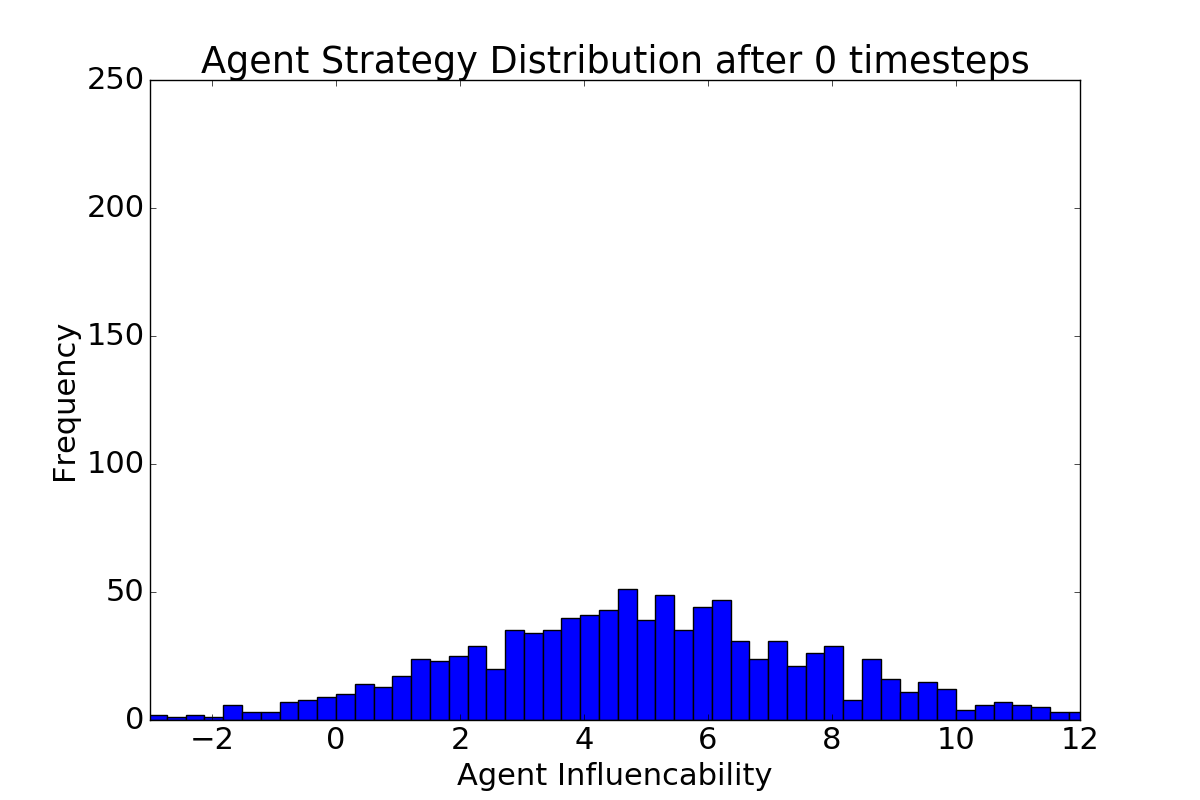
\includegraphics[width=0.45\textwidth]{figures/heuristic_gradient_example_1.png}
  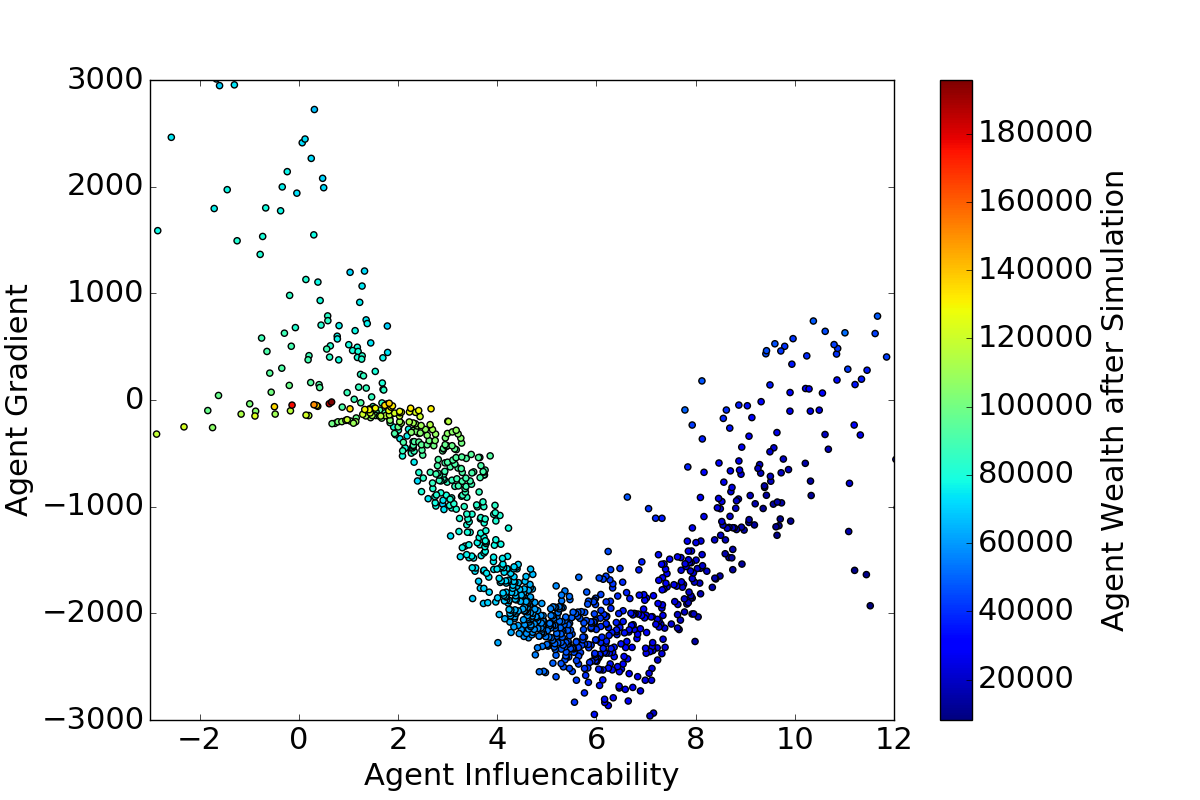
\includegraphics[width=0.45\textwidth]{figures/heuristic_gradient_example_2.png}
  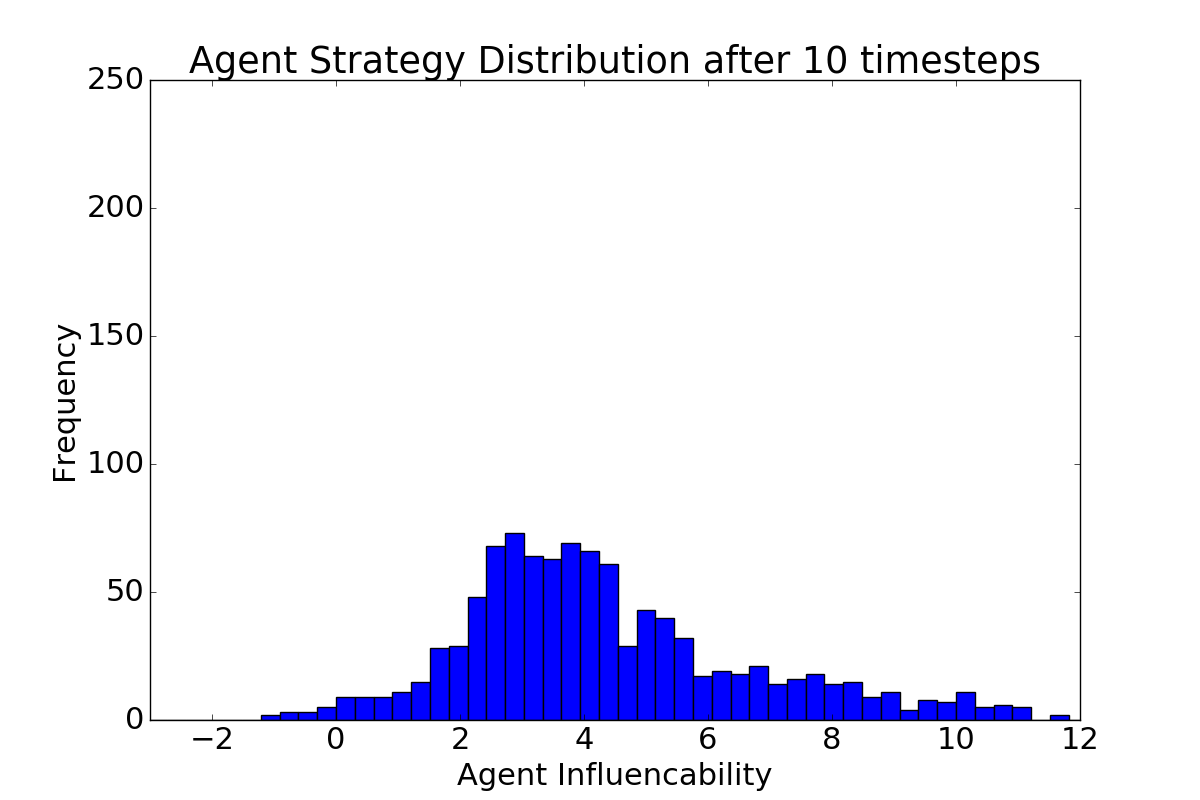
\includegraphics[width=0.45\textwidth]{figures/heuristic_gradient_example_3.png}
  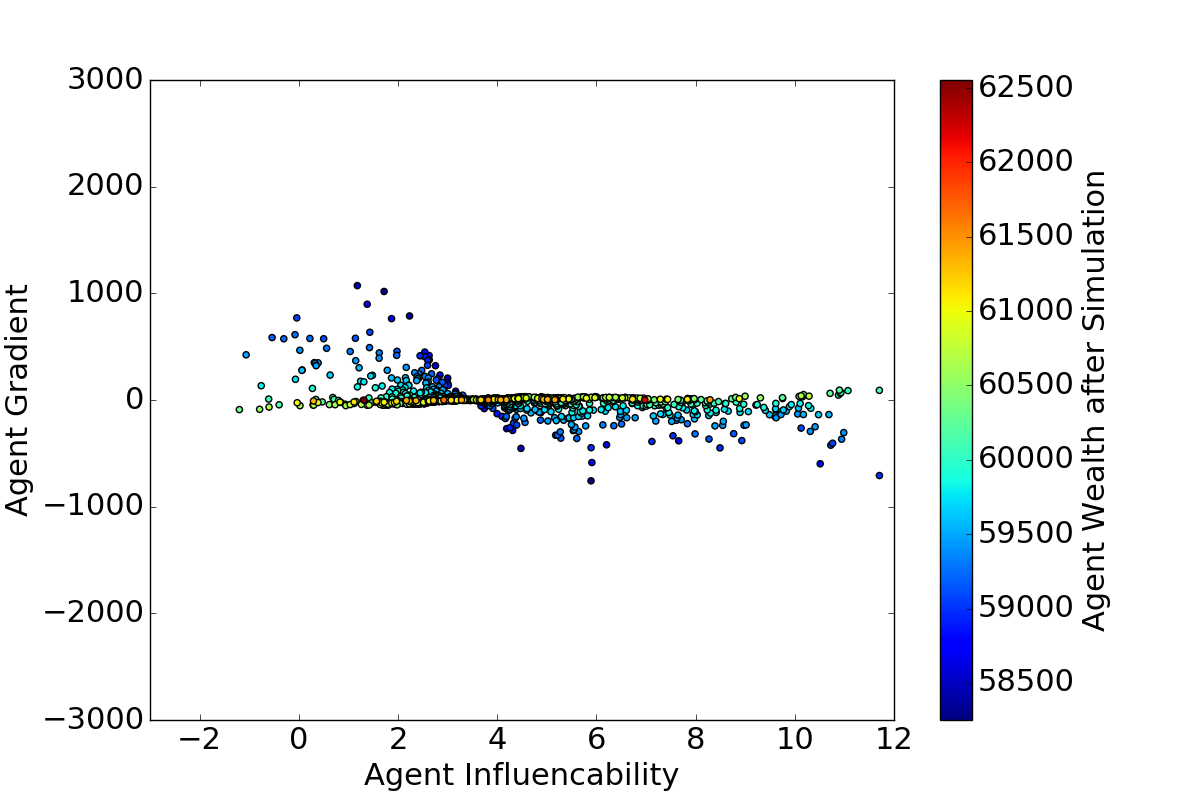
\includegraphics[width=0.45\textwidth]{figures/heuristic_gradient_example_4.png}
  \caption[Examples Heuristic Gradient]{Two examples where the simulation was run for a given 1D agent strategy distribution (left) and the corresponding agent gradients were computed (right). In the first example one can clearly see most agents having a negative gradient as the most successful agents were the ones with smallest influenceability. The second example shows a more symmetric gradient distribution.}
  \label{fig:heuristicgradient}
\end{figure}

\section{Implementation}

We implemented the above methods in Python. We used $N=1000$ agents and $T=3000$ timesteps per simulation, repeated over $L=300$ learning steps (which was generally sufficient to show convergence). Our agents each started with $M=30000$ money and $A=300$ of the tradeable asset, valued at $p_0^*=100$. Each simulation step has a runtime that is approximately linear in the number of agents (taking around 1 minute to complete all $T$ steps), while the optimisation step is somewhat more complicated. The entire process takes around 10 hours to complete, and our full experiments were run on the ETH Z\"urich Euler cluster (Intel Xeon E5-2680 CPUs).

\section{Simulation Results and Discussion}

\subsection{Single Simulation}

For clarity, we illustrate the results of a single simulation step in this section, although we repeated this process many times in the final result. \Fref{fig:singleStep} shows the buy/sell curves at selected time steps, and the price evolution over a single simulation. Qualitative observations, such as the periodic behaviour of the market due to the trade off between mean reversion and trend-following, suggest that this market behaves in a realistic way. From this premise, we performed a series of learning experiments.
\begin{figure}
  \centering
  \quad
  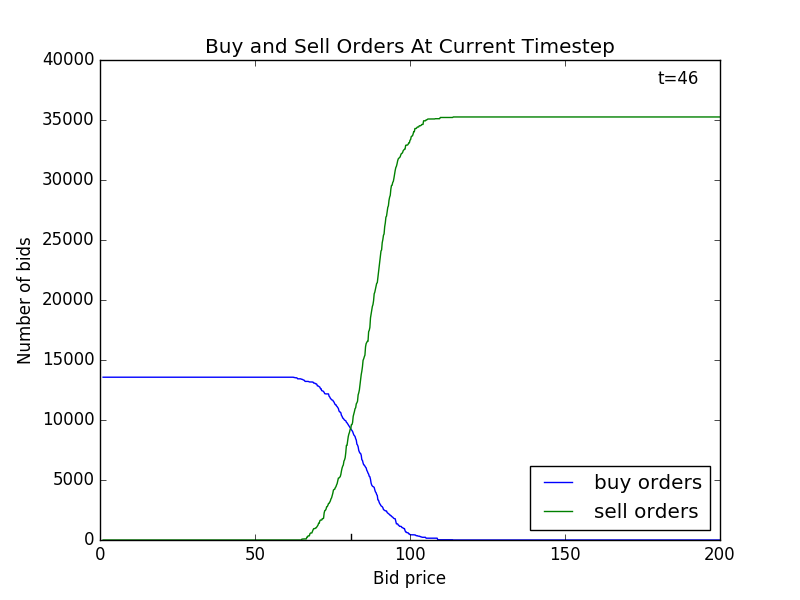
\includegraphics[width=0.31\textwidth]{figures/buy_sell_0046.png}
  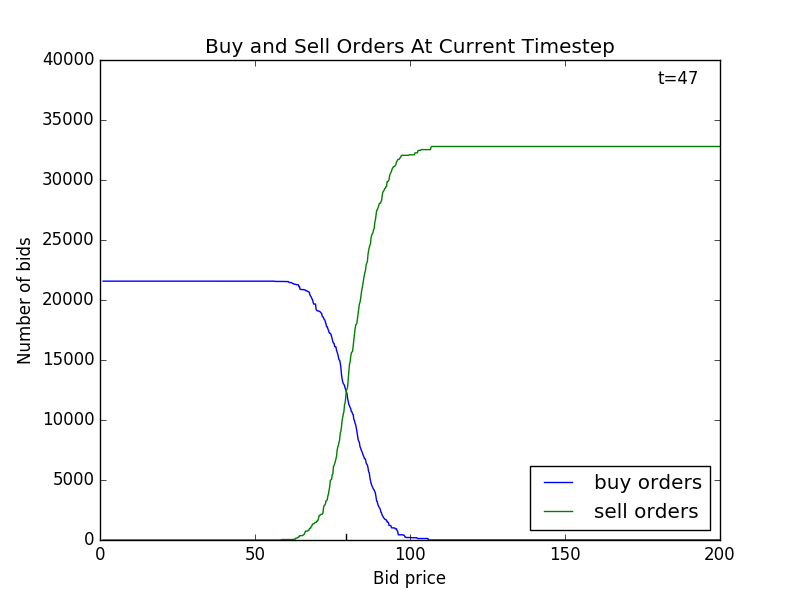
\includegraphics[width=0.31\textwidth]{figures/buy_sell_0047.png}
  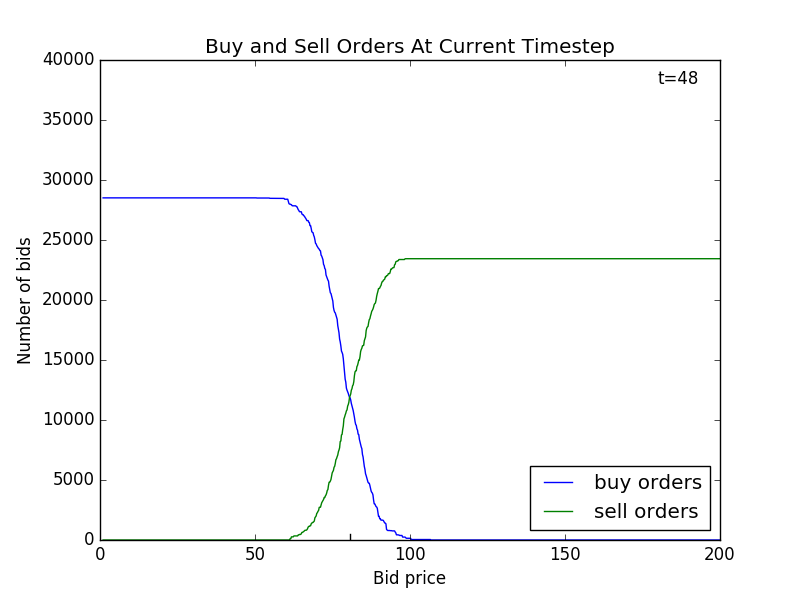
\includegraphics[width=0.31\textwidth]{figures/buy_sell_0048.png}
  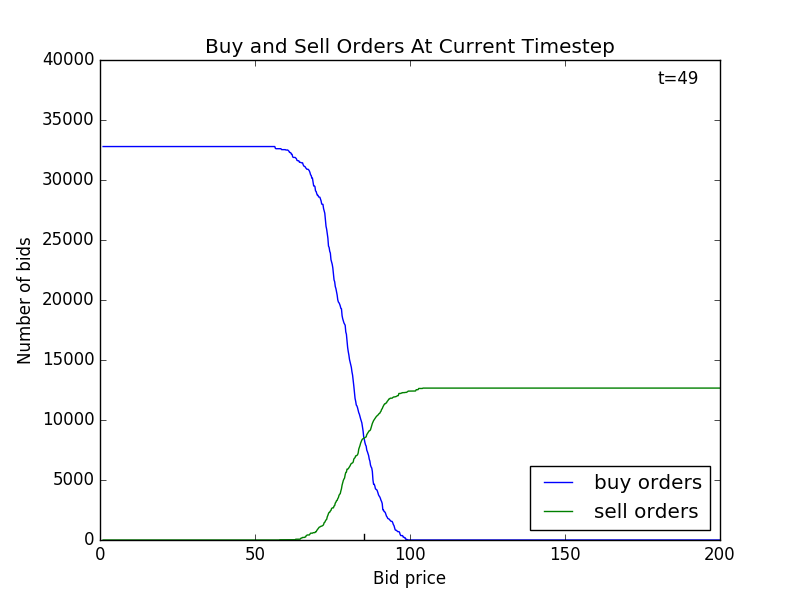
\includegraphics[width=0.31\textwidth]{figures/buy_sell_0049.png}
  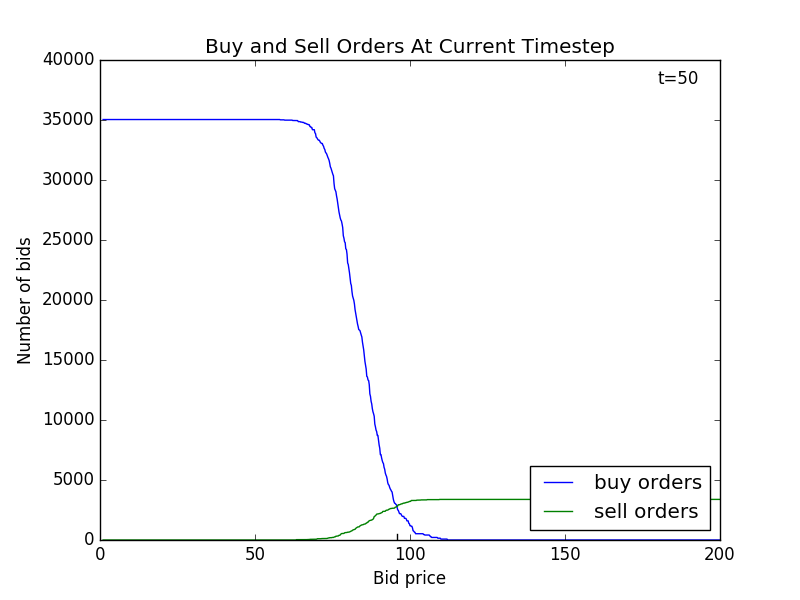
\includegraphics[width=0.31\textwidth]{figures/buy_sell_0050.png}
  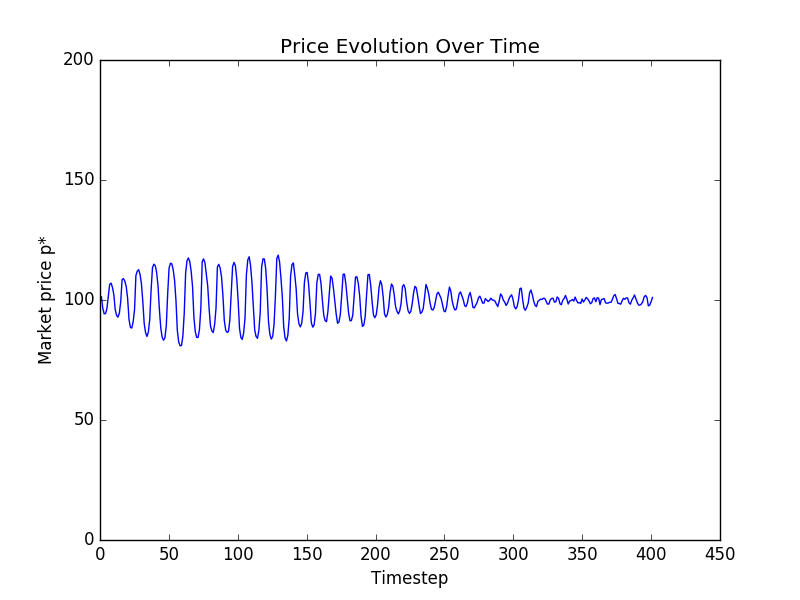
\includegraphics[width=0.31\textwidth]{figures/price_history.png}
  \caption[Price Evolution]{Buy/sell curves from 5 consecutive timesteps ($t=46$ to $t=50$). This selection shows a rise in demand and drop in supply, resulting in a price increase. The price intersections were calculated and plotted over 400 timesteps in the bottom right figure.}
  \label{fig:singleStep}
\end{figure}

\subsection{Results of Agent Learning}
Running MLS turns out to be computationally very expensive. The amount of time steps needed to reach an equilibrium distribution was about the same for the few examples we ran (as can be seen in figure \ref{fig:heuristicvsmls}), but the computation time was much longer. Thus in the scope of this project we decided to use the Heuristic Gradient method, as simulation times using Heuristic Gradient were very lengthy already. \\
\begin{figure}
  \centering
  \quad
  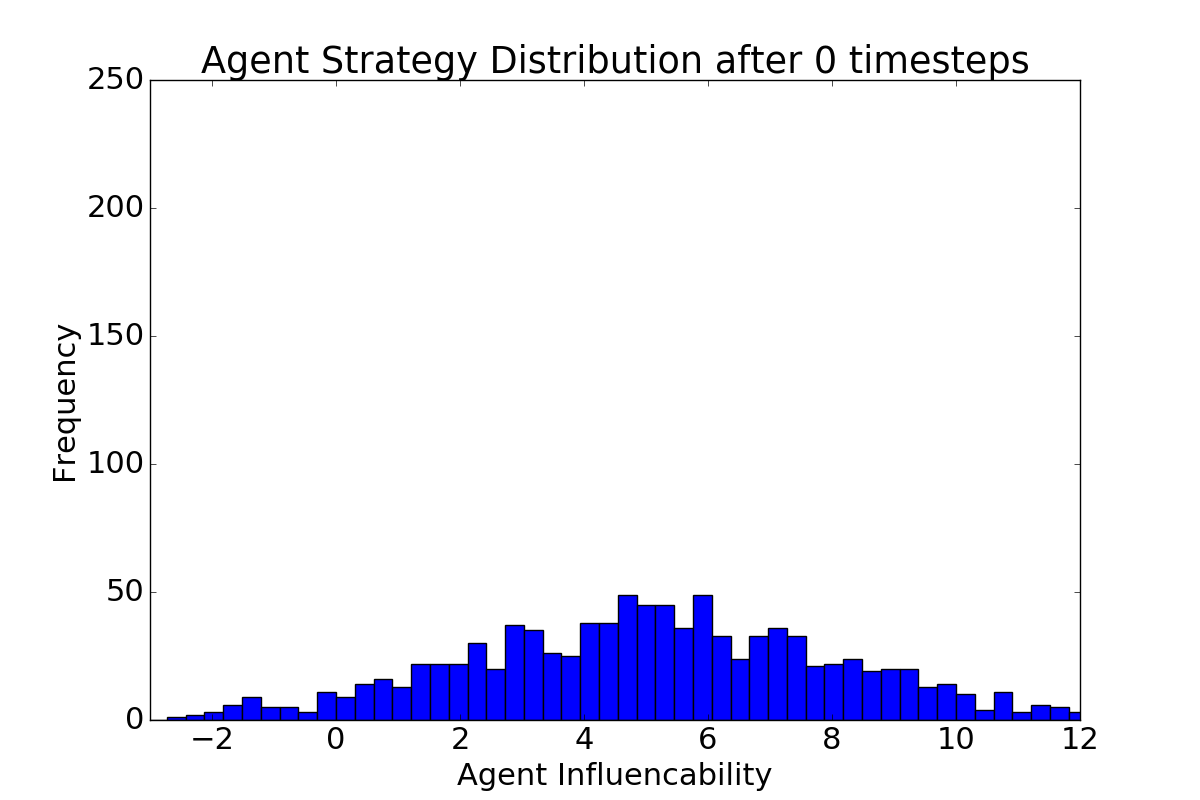
\includegraphics[width=0.45\textwidth]{figures/heuristic_vs_mls_1.png}
  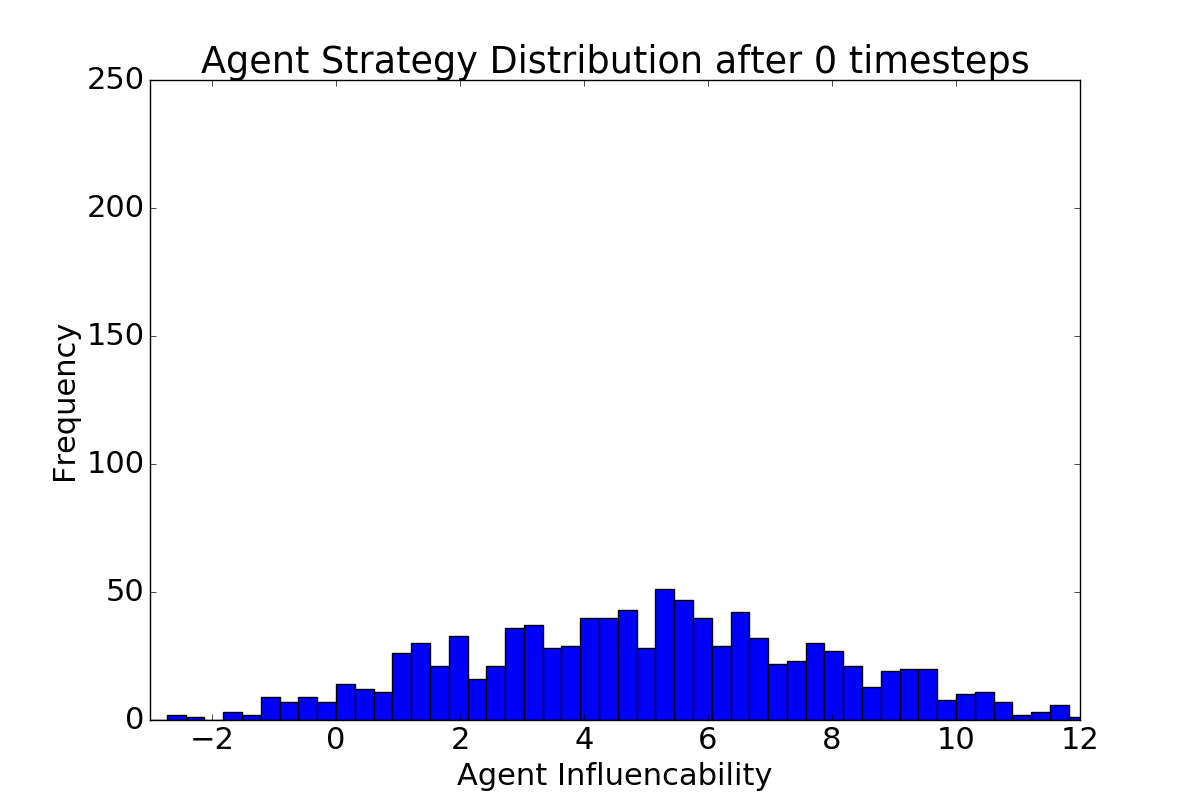
\includegraphics[width=0.45\textwidth]{figures/heuristic_vs_mls_4.png}
  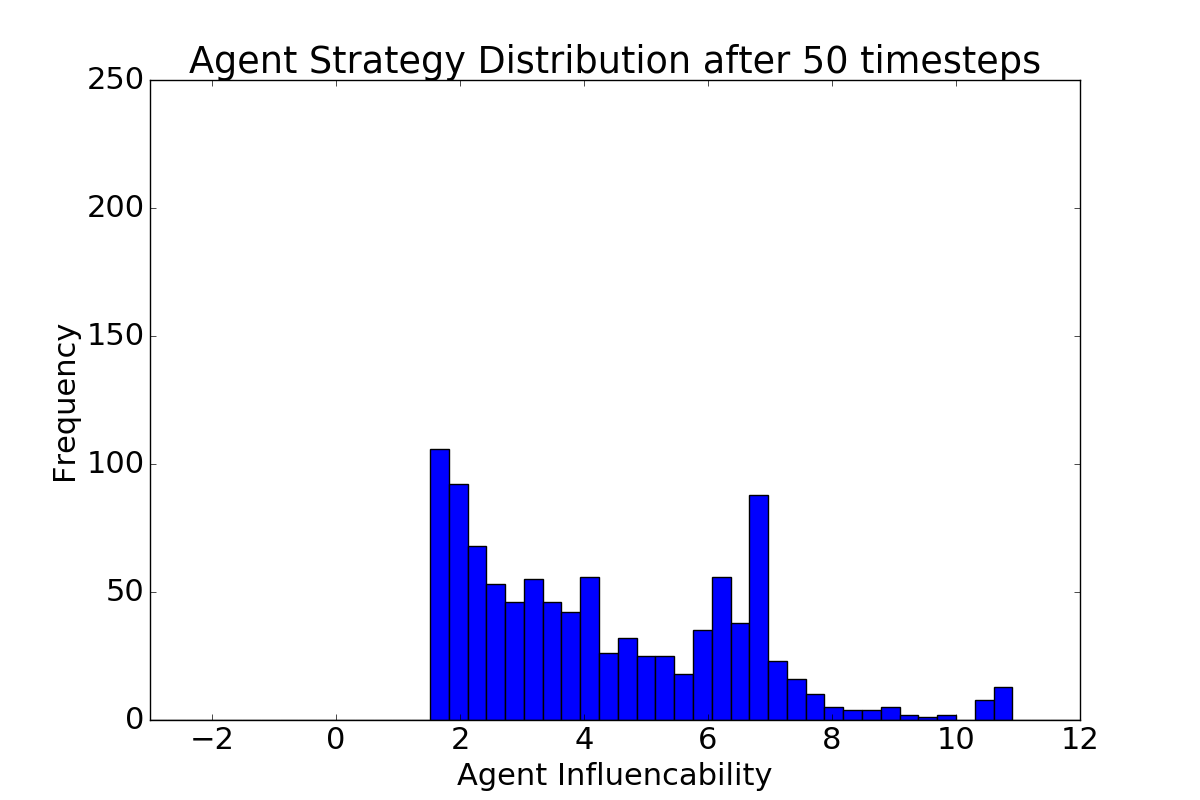
\includegraphics[width=0.45\textwidth]{figures/heuristic_vs_mls_2.png}
  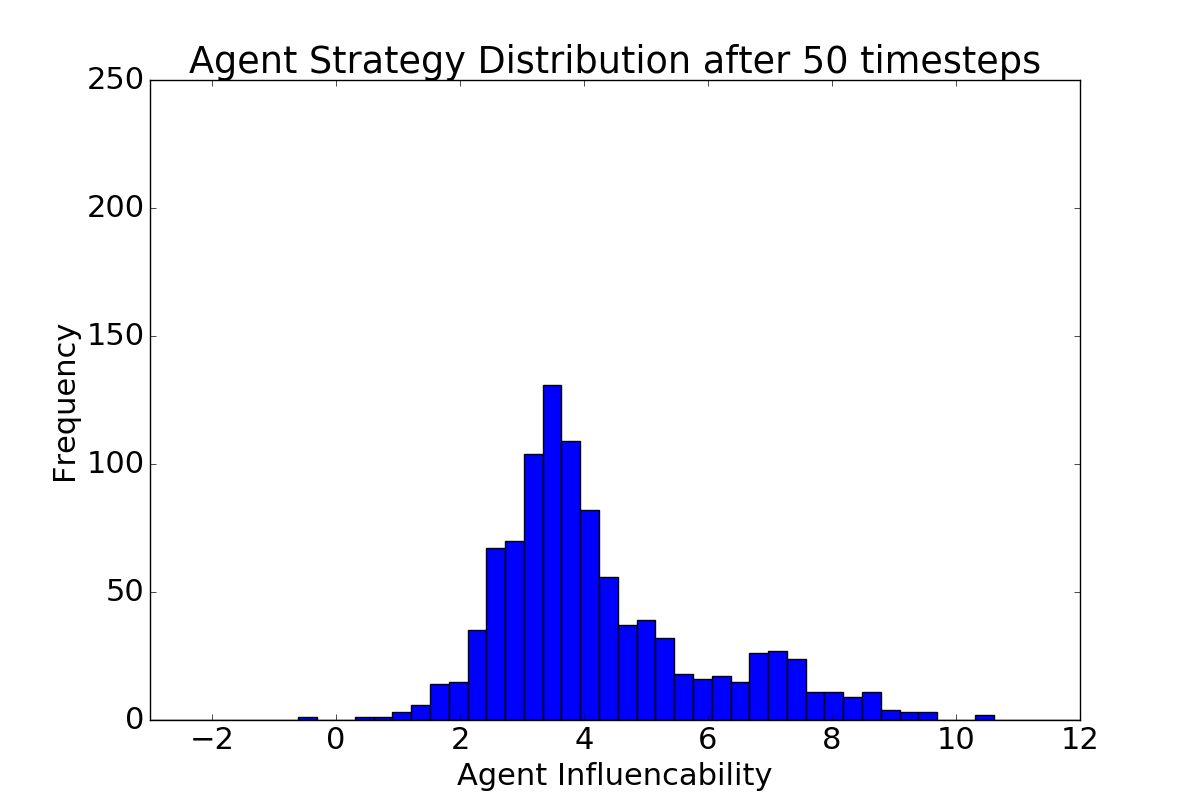
\includegraphics[width=0.45\textwidth]{figures/heuristic_vs_mls_5.png}
  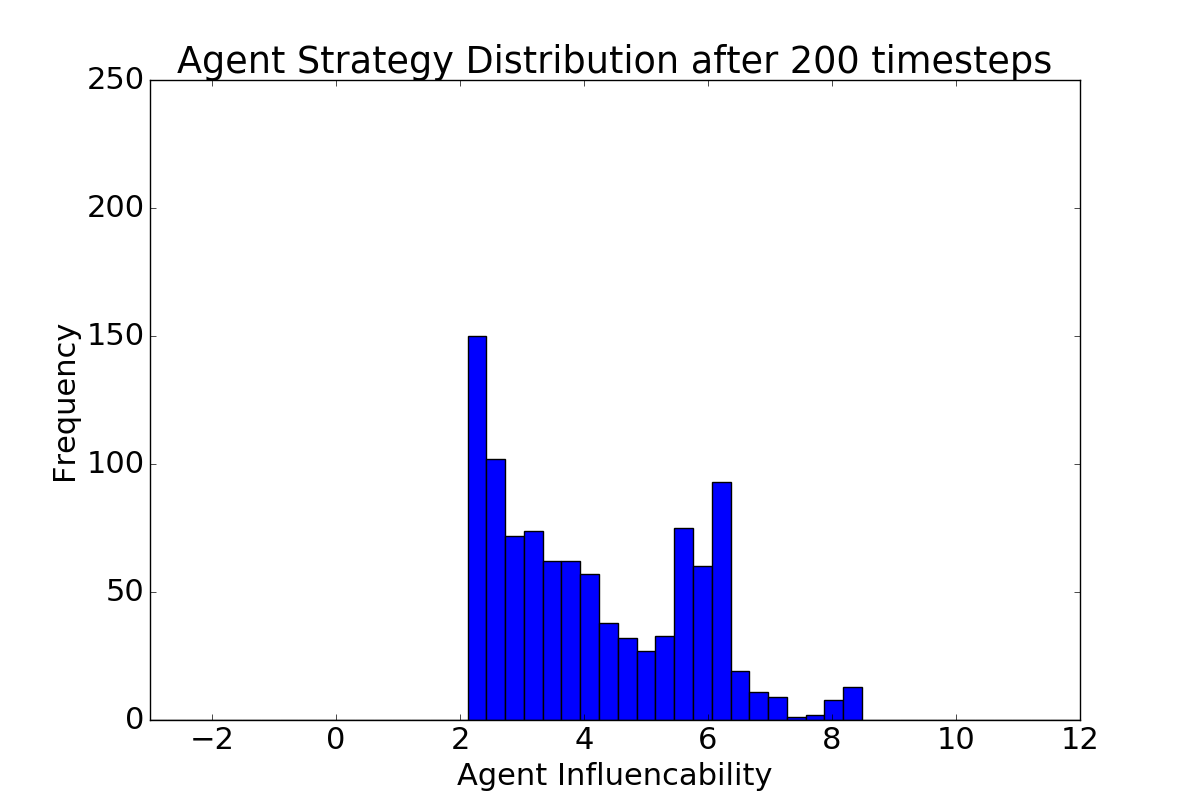
\includegraphics[width=0.45\textwidth]{figures/heuristic_vs_mls_3.png}
  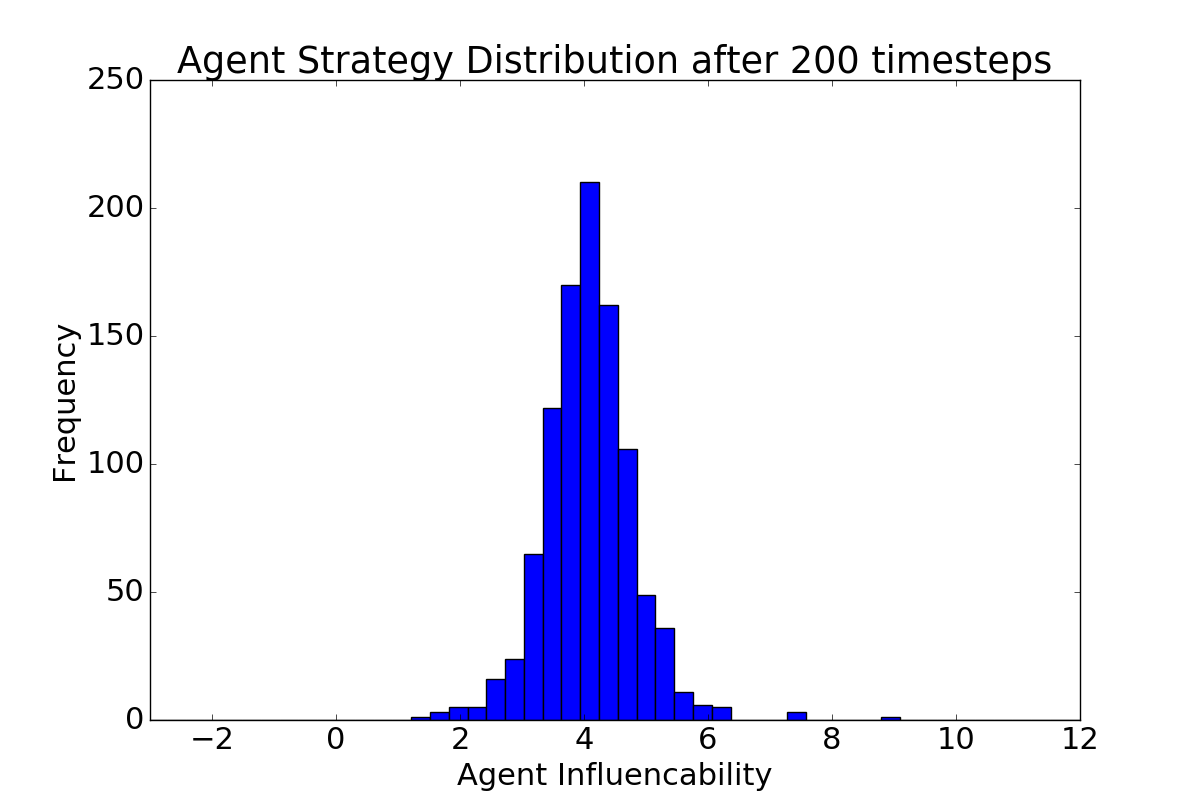
\includegraphics[width=0.45\textwidth]{figures/heuristic_vs_mls_6.png}
  \caption[Comparison MLS and Heuristic Gradient]{Simulation result of the MLS (left) and Heuristic Gradient (right) methods for the same initial agent distributions after 0, 50 and 200 timesteps. Both methods reached a stable distribution at around 150 timesteps.}
  \label{fig:heuristicvsmls}
\end{figure}
Additionally it was decided to reduce the agent parameter space to one dimension, as 2D (or even 3D simulation if the agent noisiness is not fixed) simulations need more learning steps and/or lower learning parameter. This can be seen in figure \ref{fig:2dsimulation} where a 2D simulation was run for 1000 learning steps. Even though the shrinking shape of the agent parameter distribution suggests that it would converge at some point, that point is still not reached after 1000 learning steps. \\
To reduce the parameter space to 1D we bind influenceability and conservativeness with following equation: 
\begin{equation}
  \text{conservativeness} = \frac{9 - \text{influenceability}}{400}
\end{equation}
\begin{figure}
  \centering
  \quad
  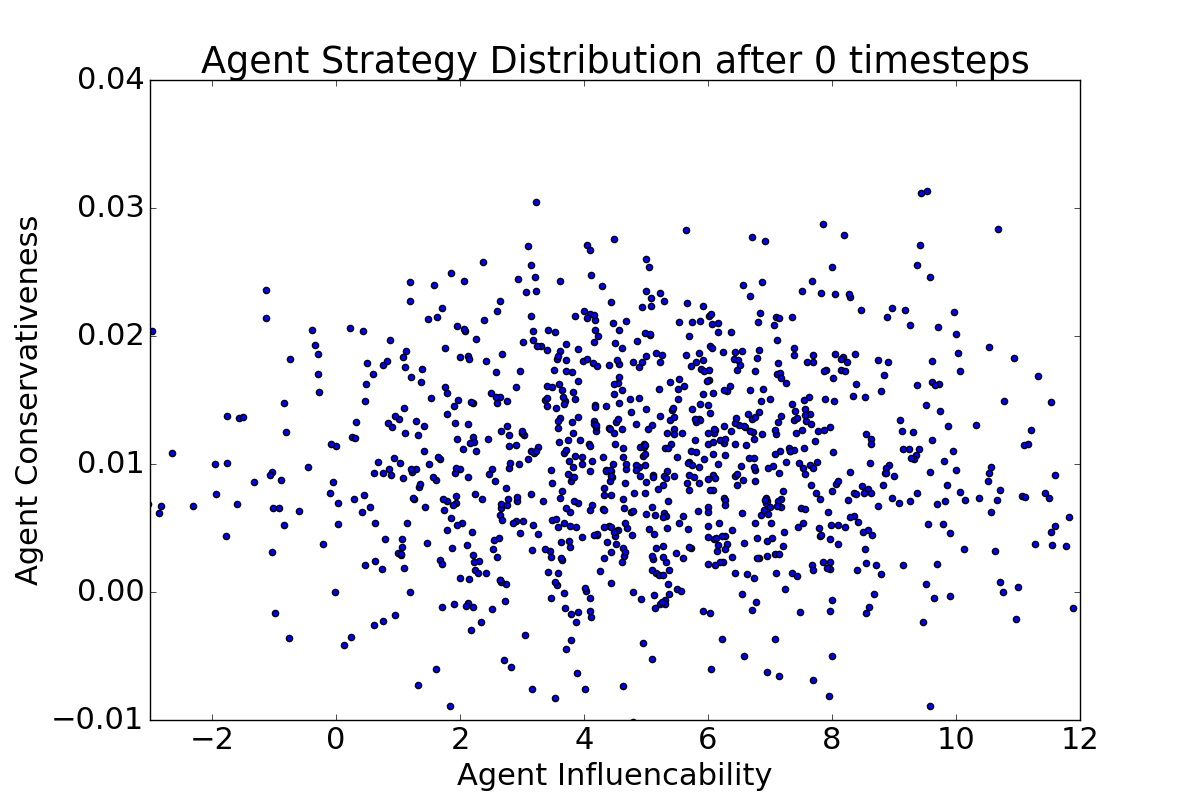
\includegraphics[width=0.31\textwidth]{figures/2dsim_1.png}
  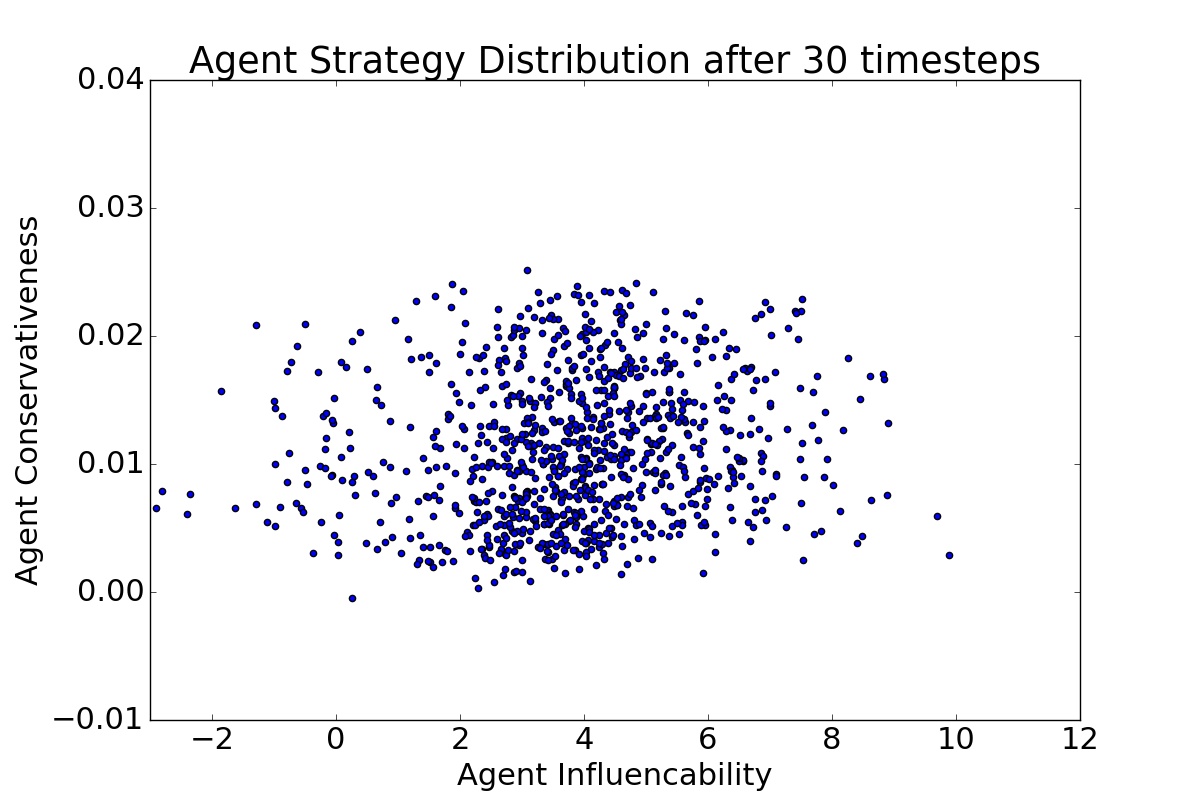
\includegraphics[width=0.31\textwidth]{figures/2dsim_2.png}
  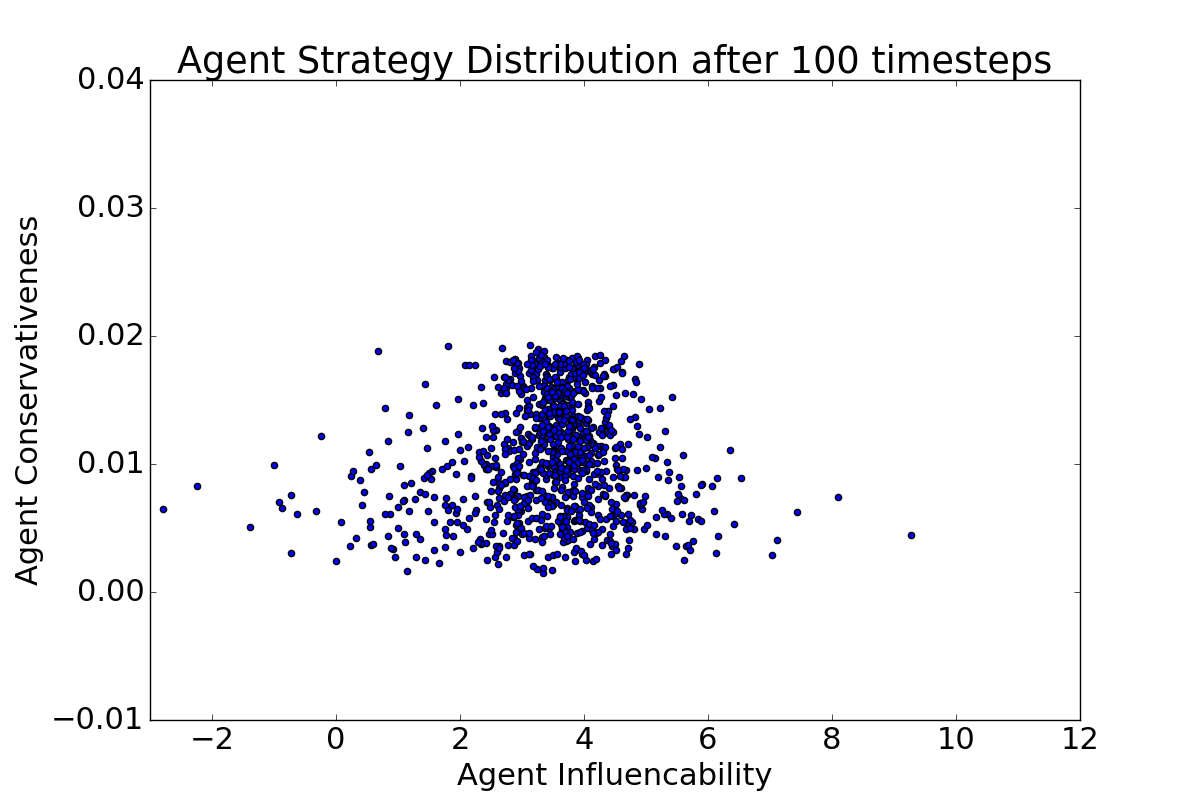
\includegraphics[width=0.31\textwidth]{figures/2dsim_3.png}
  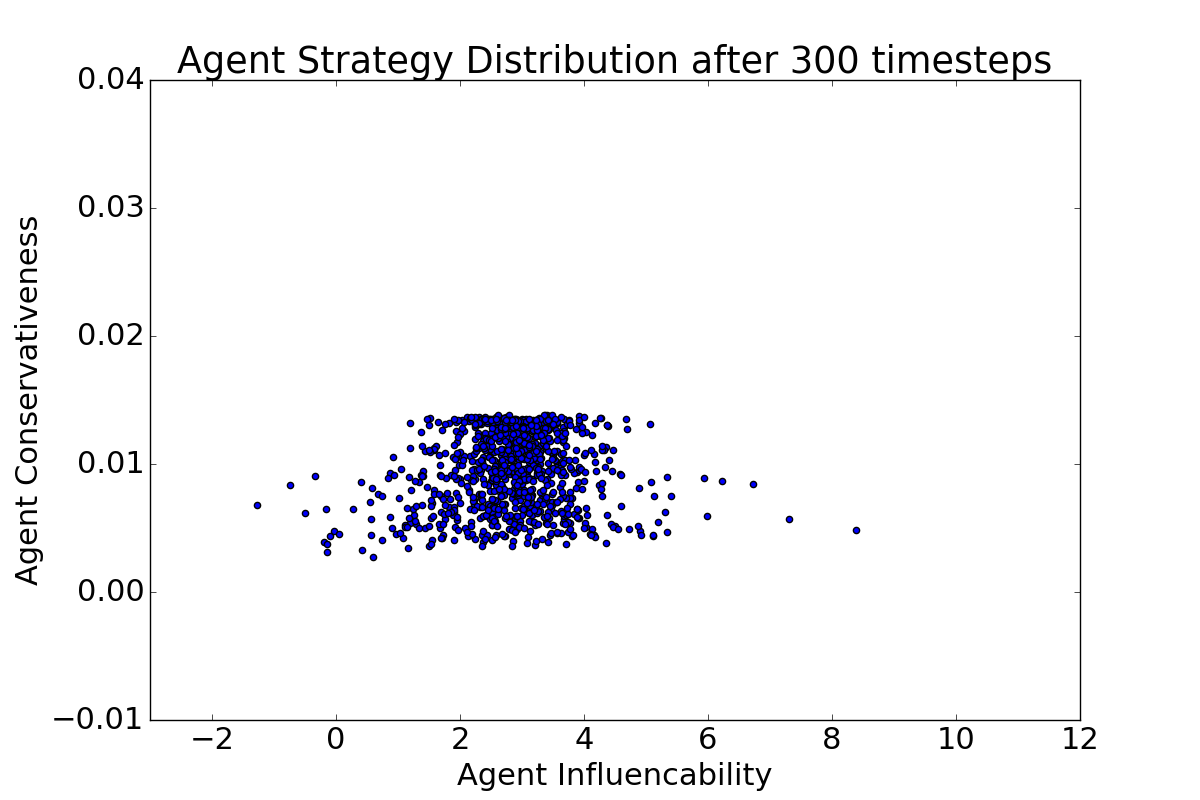
\includegraphics[width=0.31\textwidth]{figures/2dsim_4.png}
  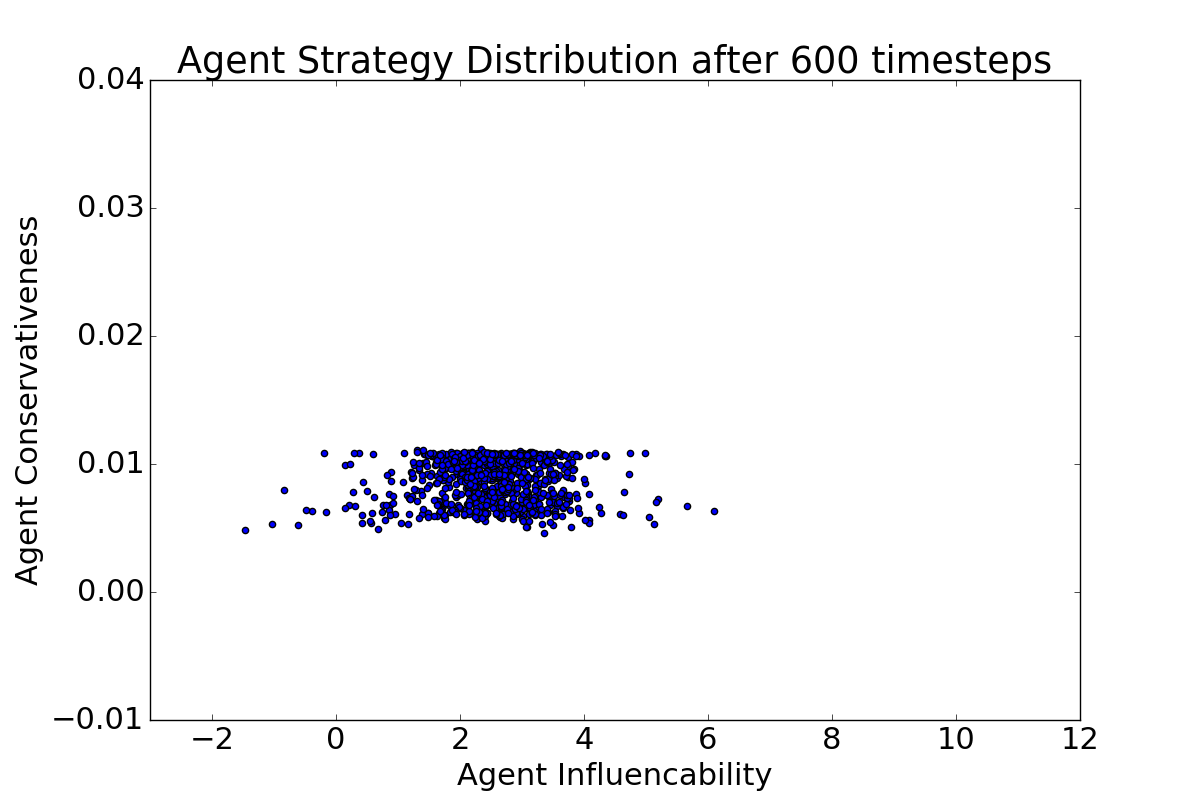
\includegraphics[width=0.31\textwidth]{figures/2dsim_5.png}
  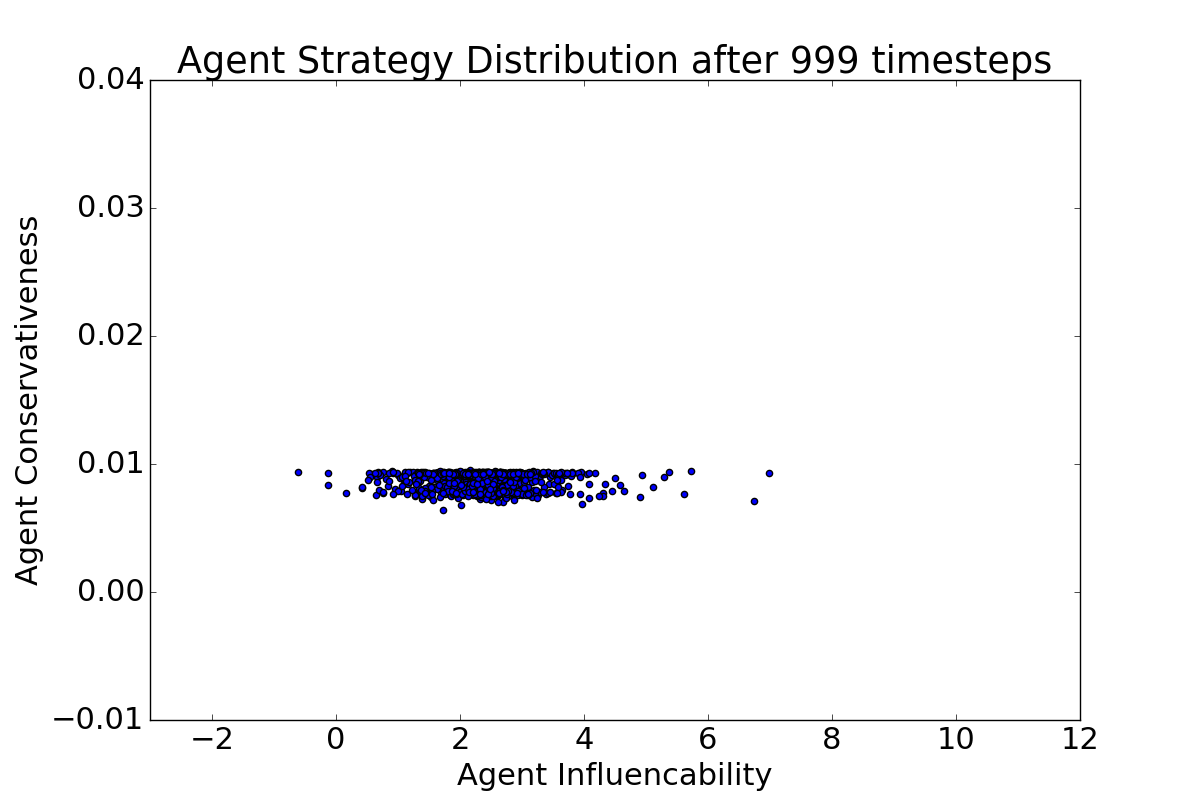
\includegraphics[width=0.31\textwidth]{figures/2dsim_6.png}
  \caption[2D simulation]{Evolution of agent parameter distribution for a Heuristic Gradient optimisation in a 2D parameter space (conservativeness and influenceability). Even after 1000 learning steps the distribution has not converged, as the shape is still changing.}
  \label{fig:2dsimulation}
\end{figure}

\hfill \\
All following simulations are done with the Heuristic Gradient method in the reduced 1D agent parameter space. One example of such a learning process is visualised in figure \ref{fig:convergenceexample}. In this case we chose a normal initial agent distribution with mean 5 and standard deviation 3. As one can see the strategy distribution converges to a stable Gaussian-like shape. This convergence behaviour is analysed if firstly it is consistently reproducible and secondly if it depends on the initial strategy distribution of the agents. \\
\begin{figure}
  \centering
  \quad
  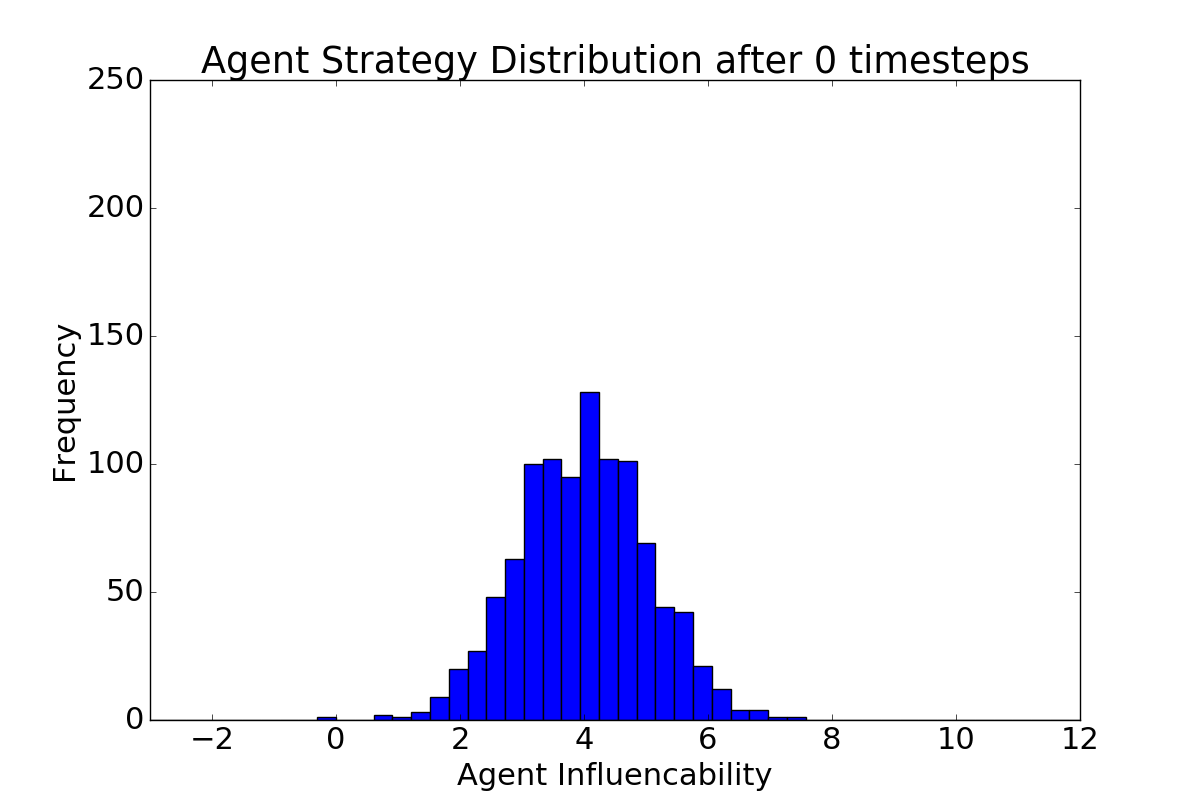
\includegraphics[width=0.45\textwidth]{figures/convergence_example_1.png}
  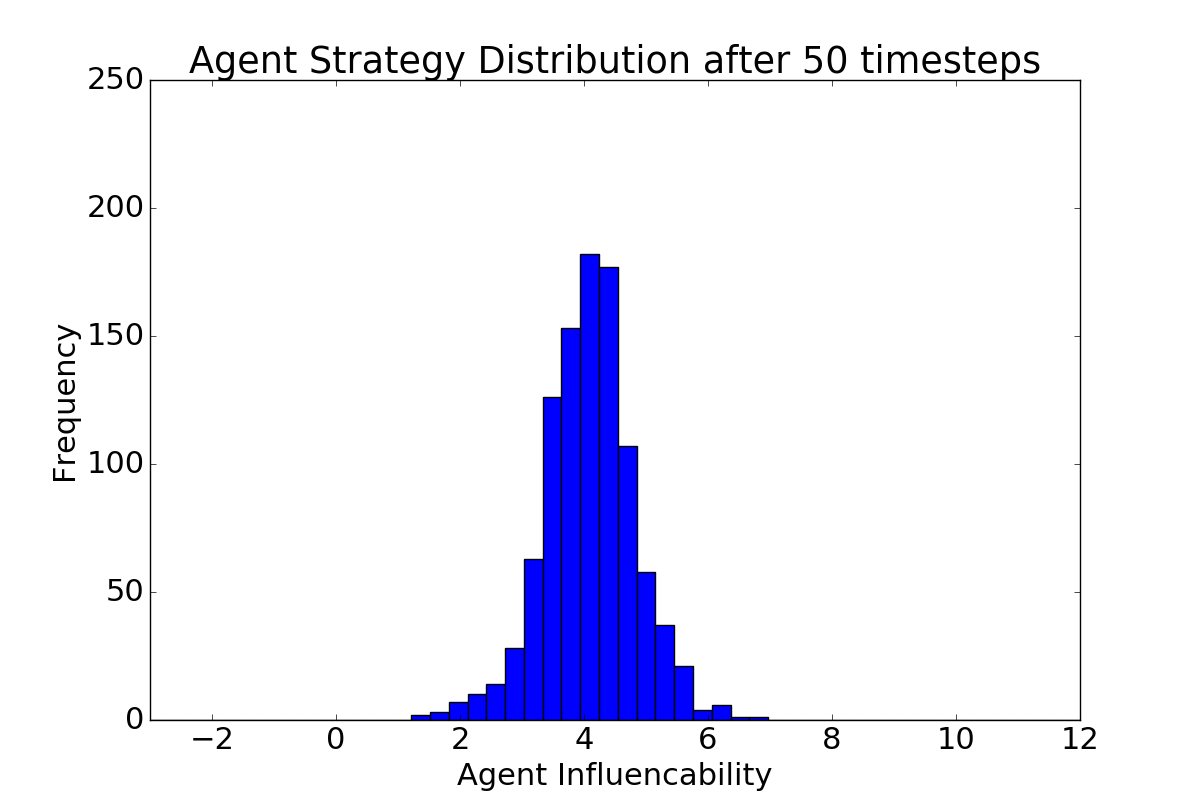
\includegraphics[width=0.45\textwidth]{figures/convergence_example_2.png}
  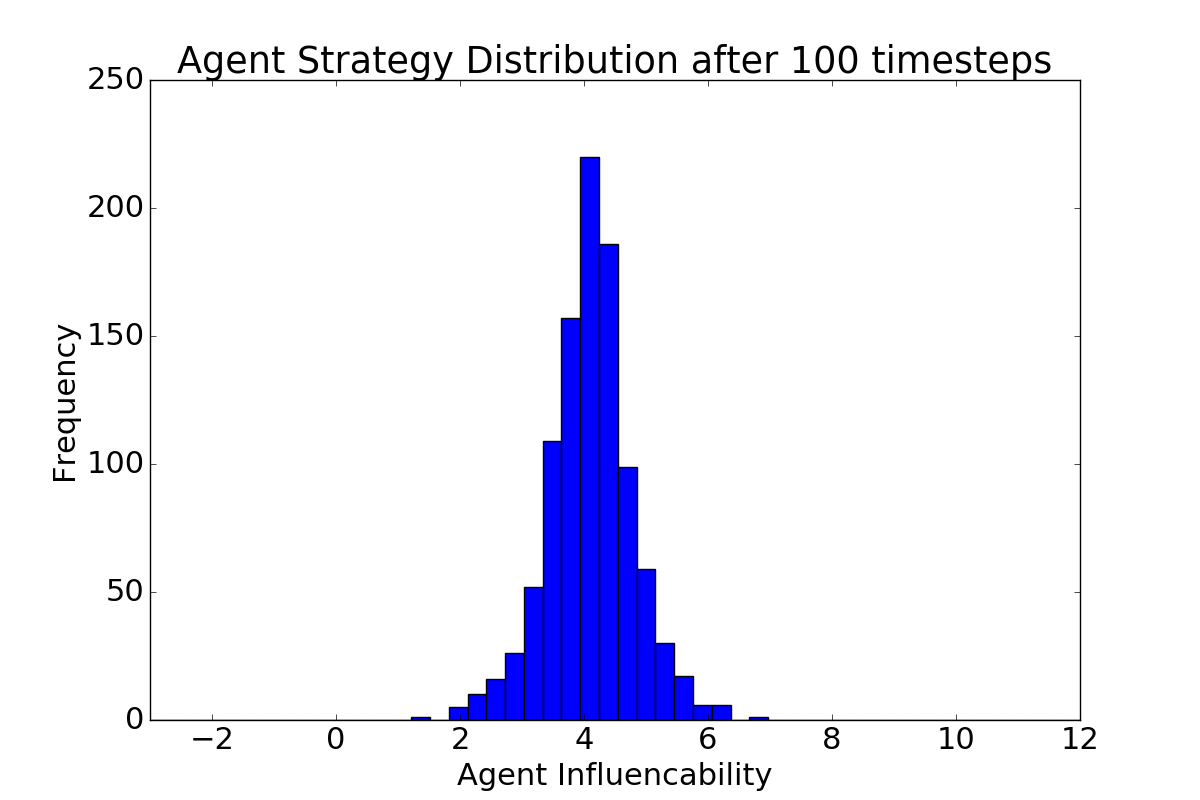
\includegraphics[width=0.45\textwidth]{figures/convergence_example_3.png}
  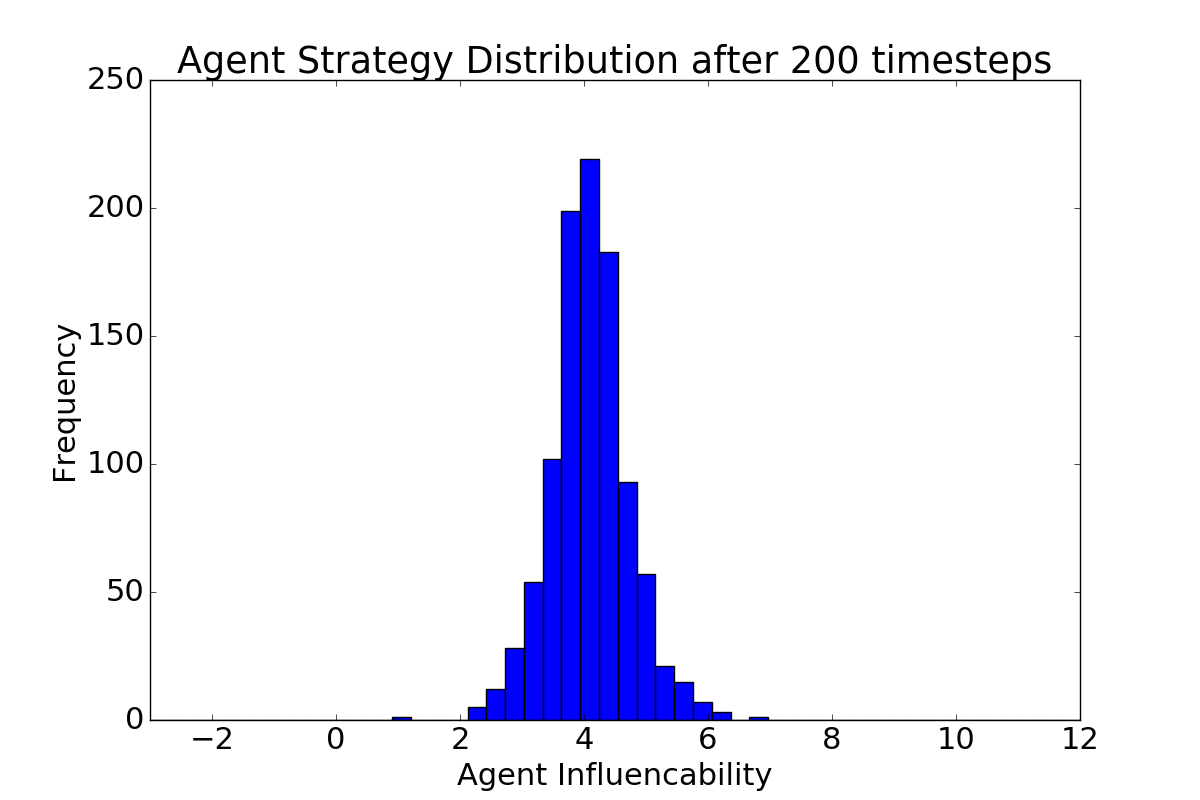
\includegraphics[width=0.45\textwidth]{figures/convergence_example_4.png}
  \caption[Convergence Example]{Results of a 1D Heuristic Gradient simulation with initial parameter distribution being normal with mean 5 and standard deviation 3. After around 100 timesteps the distribution converges to a Gaussian-like shape and stays that way.}
  \label{fig:convergenceexample}
\end{figure}
The simulation is therefore ran 10 times with the same initial distribution of agent parameters and the same Gaussian-like curve was always observed in all the final distributions. All those distributions are fitted against a Gaussian function yielding us ten different values for the mean $\mu_{conv}$ and the standard deviation $\sigma_{conv}$. Computing the standard deviation of those two sets yields the result:
\begin{center}
  $\mu_{conv} = 4.07\pm 0.03$ \\
  $\sigma_{conv} = 0.53\pm 0.02$
\end{center}
The remarkably small deviations indicate a high reproducibility of the result. This gives us an idea of the uncertainty of the simulation result given an initial set of agents. This is very useful when one intends to investigate the dependence of the simulation result on the initial agent parameter distribution as we will below. \\
\hfill \\
We ran 35 different simulations for different initial agent strategy distributions. The distributions were chosen to be normal with the mean and standard deviation being all possible permutations of $\mu=2,3,4,5,6,7,8$ and $\sigma=1,2,3,4,5$. Some of those initial distributions can be seen in figure \ref{fig:initialconditions}. They span the complete sensible space of agent parameters: Markets with high amount of agents with negative influenceability start producing nonsensical behaviour, as most agents try to do the opposite of all other agents. Similarly markets with many agents with influenceability larger than 15 were observed to crash quickly, as price immediately fell down to zero or skyrocketed to unreasonable values. \\
\begin{figure}
  \centering
  \quad
  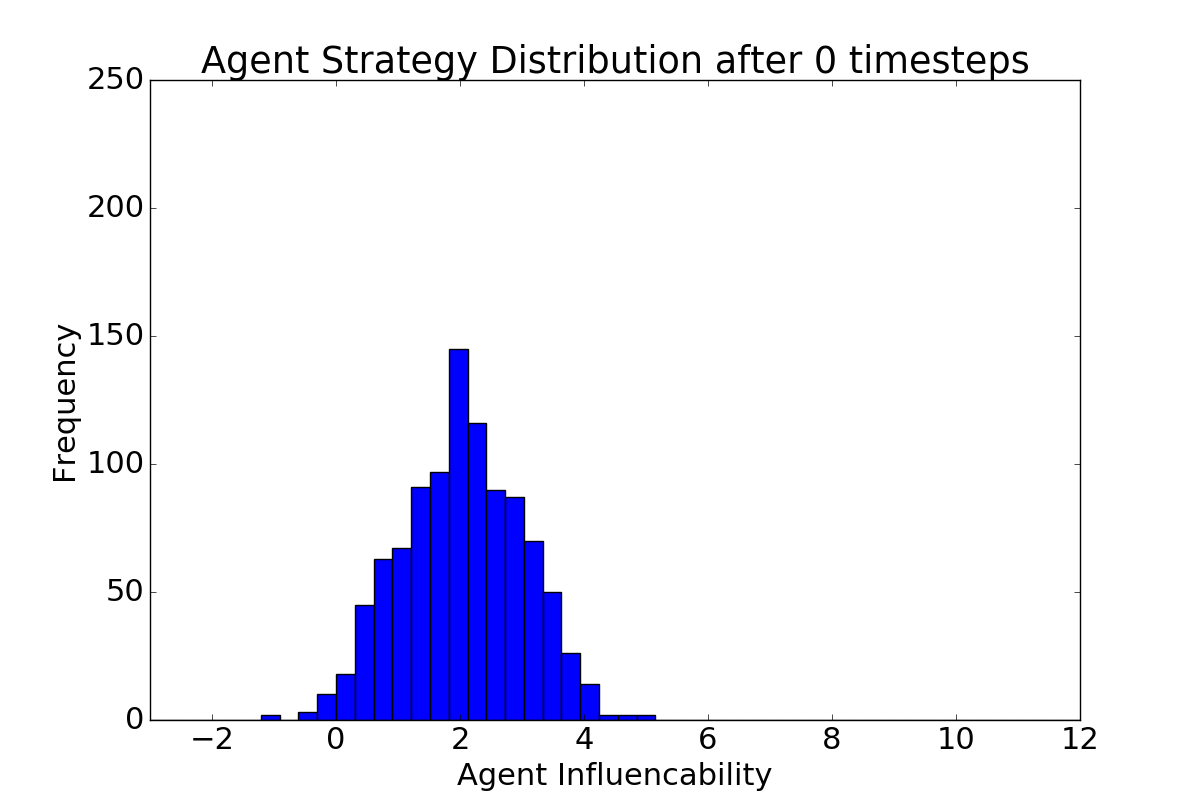
\includegraphics[width=0.3\textwidth]{figures/ic1.png}
  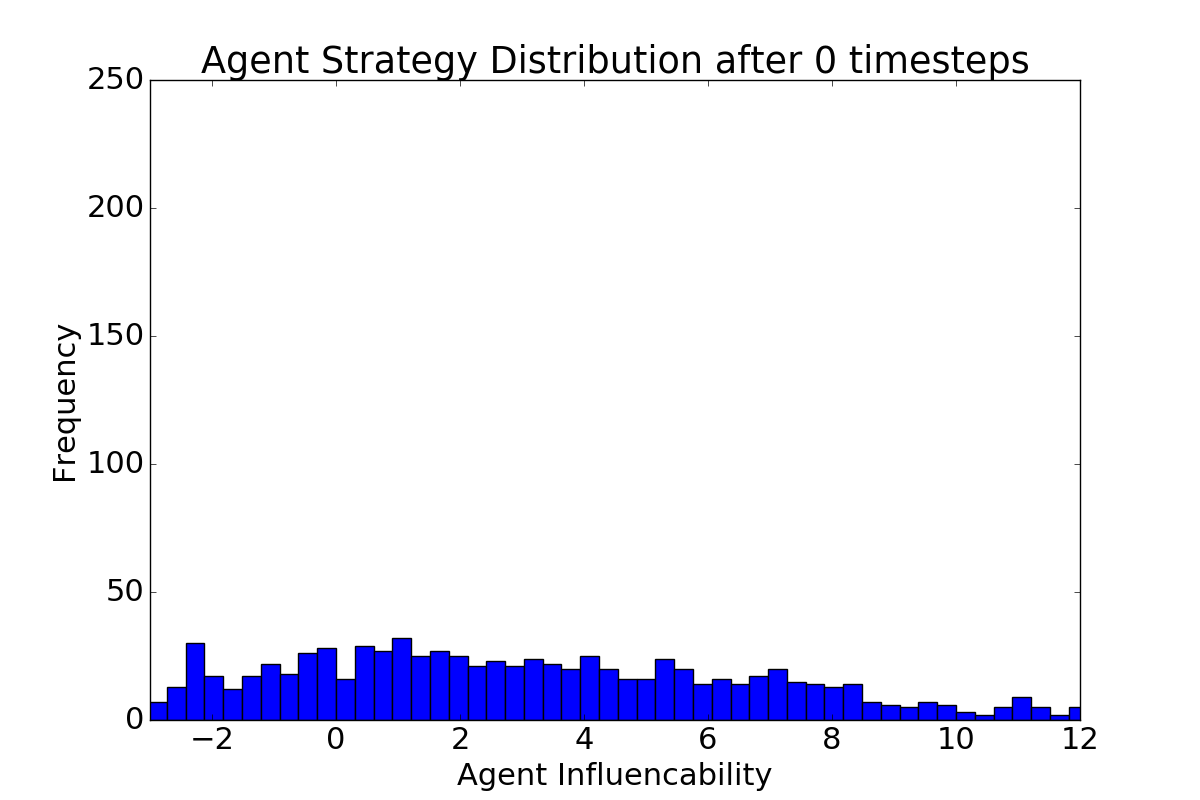
\includegraphics[width=0.3\textwidth]{figures/ic2.png}
  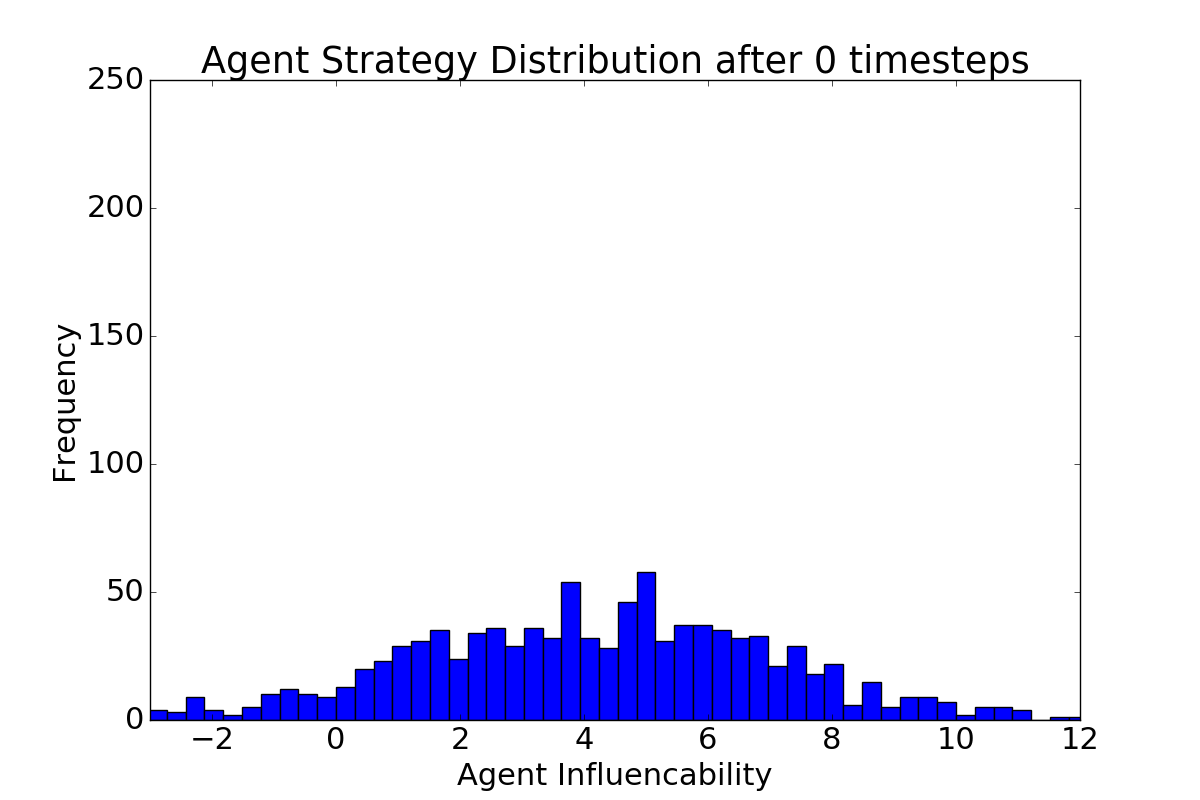
\includegraphics[width=0.3\textwidth]{figures/ic3.png}
  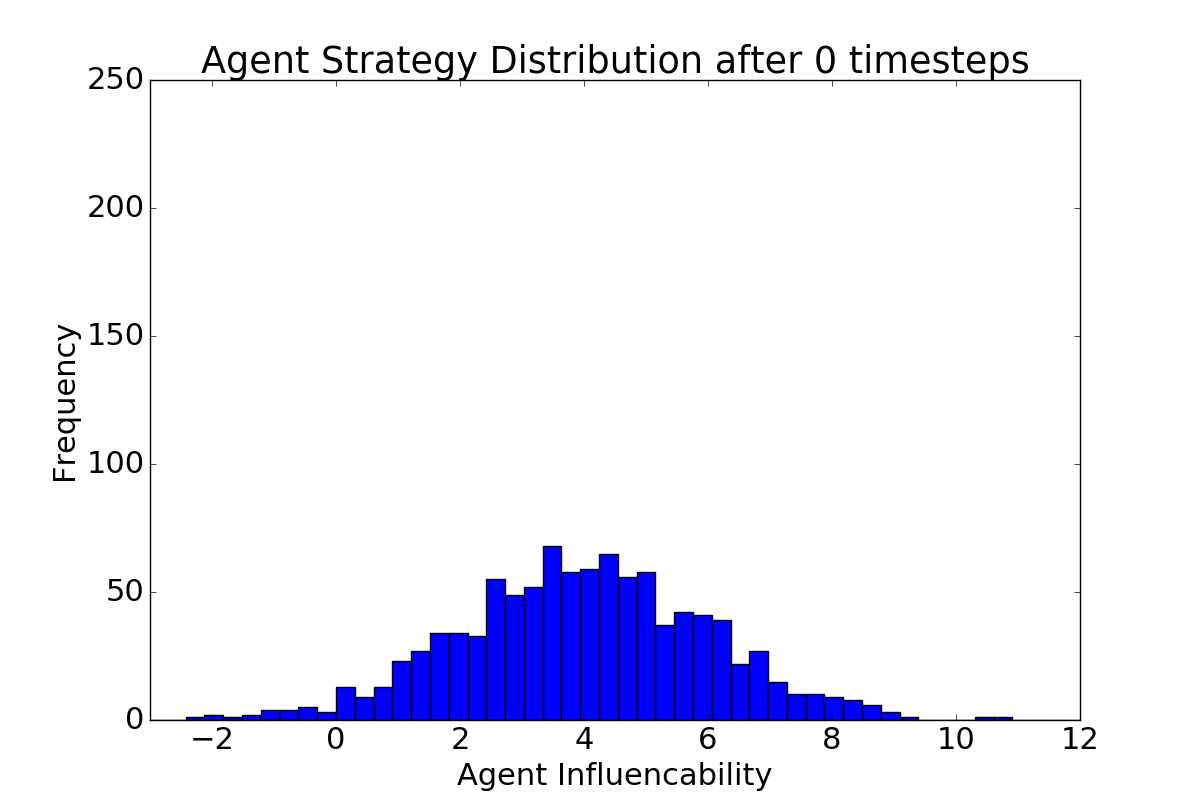
\includegraphics[width=0.3\textwidth]{figures/ic4.png}
  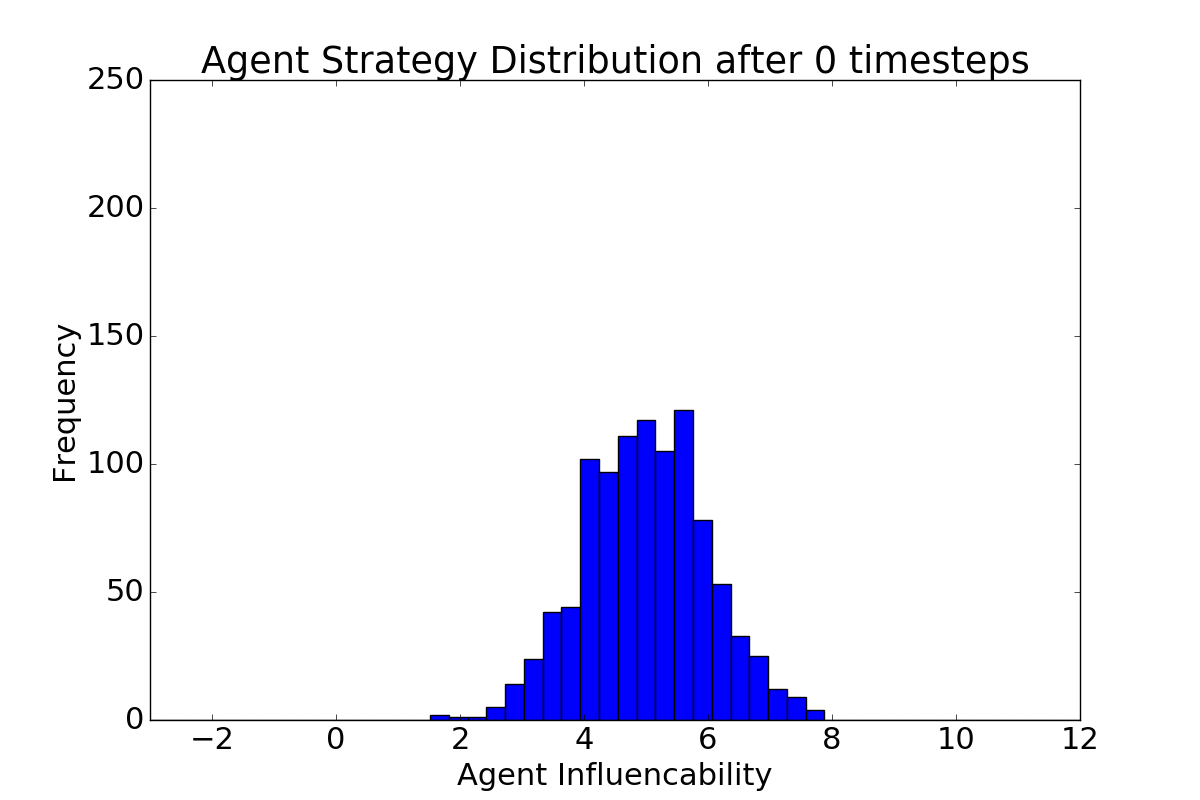
\includegraphics[width=0.3\textwidth]{figures/ic5.png}
  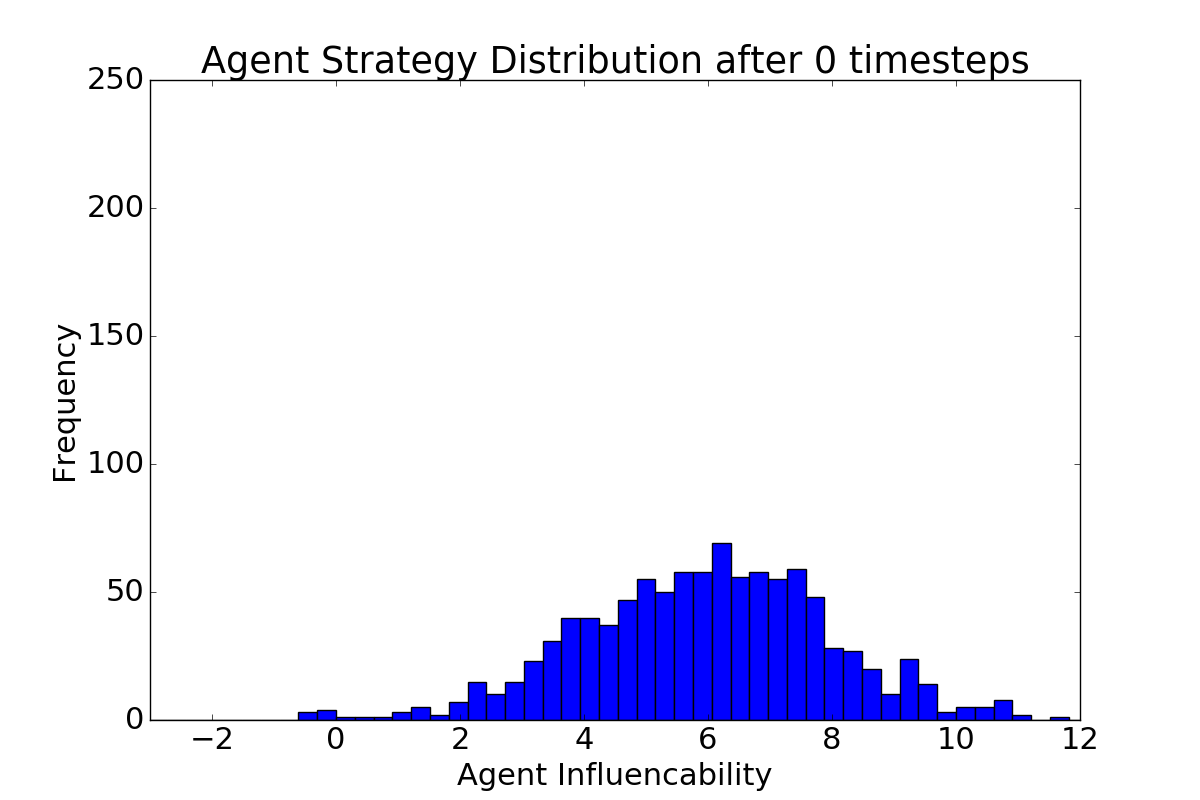
\includegraphics[width=0.3\textwidth]{figures/ic6.png}
  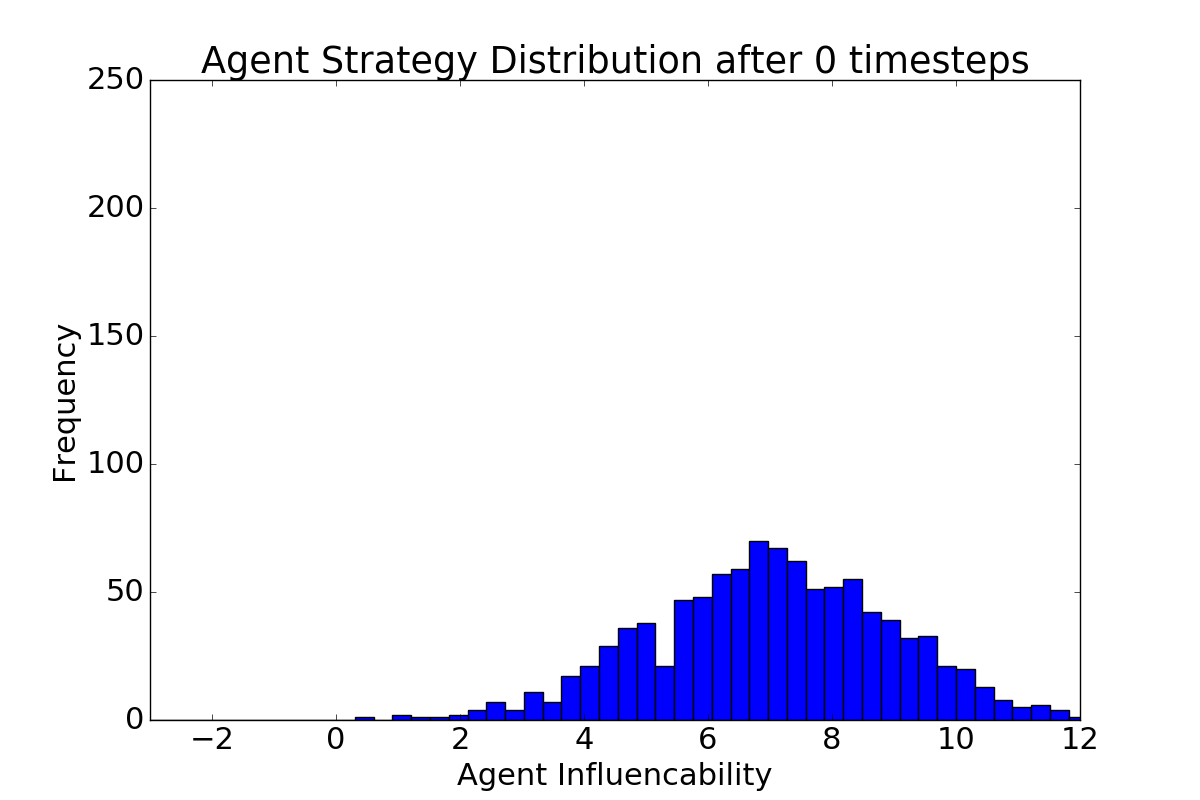
\includegraphics[width=0.3\textwidth]{figures/ic7.png}
  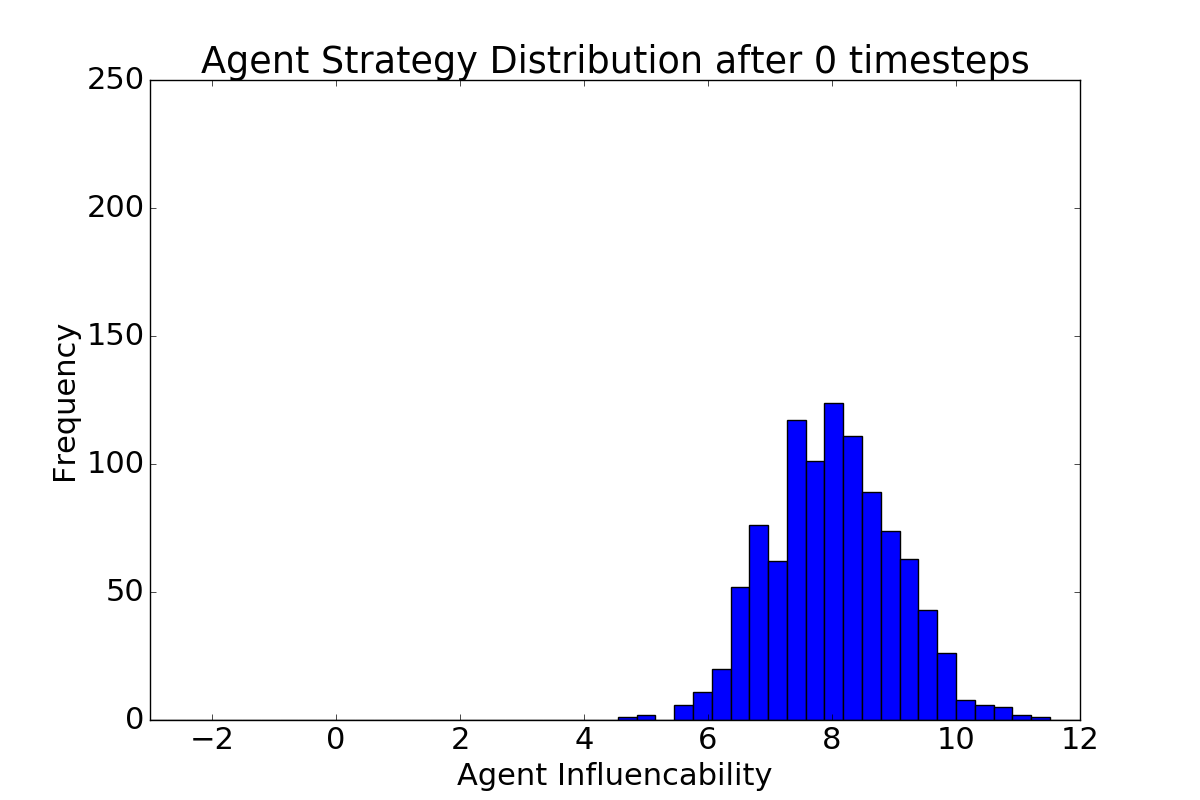
\includegraphics[width=0.3\textwidth]{figures/ic8.png}
  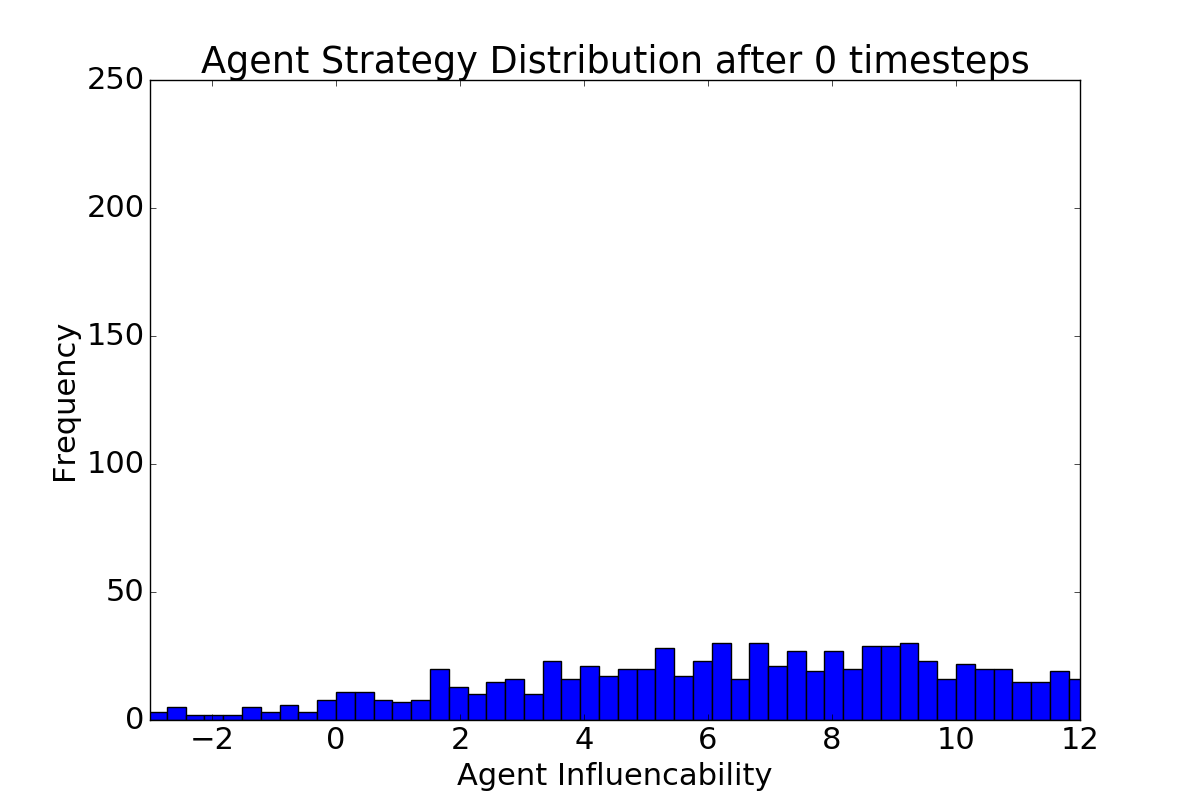
\includegraphics[width=0.3\textwidth]{figures/ic9.png}
  \caption[Different Initial Conditions]{9 of the 35 tested initial agent strategy distributions are plotted.}
  \label{fig:initialconditions}
\end{figure}
For all 35 different initial conditions the agent distribution converged to the same Gaussian-like curve. Analogously as before those final histograms were fitted against a normal distribution resulting in
\begin{center}
  $\mu_{conv} = 4.09\pm 0.07$
  $\sigma_{conv} = 0.52\pm 0.03$
\end{center}
These numbers are very similar to those observed in the reproducibility experiment, leading to the conclusions that our system always converges to the same strategy distribution.

\section{Summary and Outlook}
First we developed an agent-based model for financial market that is able to produce a wide variety of agent behaviour by introducing three agent parameters. We investigated an strategy optimisation process for a reduced agent parameter space that converged consistently to the same strategy distribution, independent of the initial distribution in a sensible range of initial agent parameters. This result is quite remarkable, as such a consistent outcome was not certain before running the simulations. However the precise shape of such an equilibrium distribution depends on the optimisation process used. For example if the learning parameter were increased, one would expect the width of the equilibrium distribution to increase. Still there is an intrinsic property of our model independent on the learning algorithm that one can extract from our result: If the strategy distribution in a market adopts the Gaussian-like shape that we discovered, then the ideal strategy for an agent is to appropriate the parameter value at the mean of the curve. Therefore we have in a certain way found an optimal strategy for the system. \\
\hfill \\
There are however still many areas that warrant further investigation of our model and our optimisation process:
\begin{itemize}
  \item The restriction of the agent parameter space from 3D to 1D is completely arbitrary. Ideally one would want to run the optimisation in all parameters, but this necessitates more computational power and time than available to us for our project.
  \item The optimisation process should be investigated more thoroughly. It is not a typical optimisation process where one wants to find the extrema of a multivariate fitness function, because of two reasons: The output of our fitness function is stochastic and strongly depends on the other agents. The fitness function therefore changes slightly at each learning step as all the other agents change their parameters thus changing the market dynamics. Our optimisation method naively ignores this fact. Therefore further research for more suitable mathematical methods is necessary.
  \item Our current result do not justify why our model and our optimisation approach are sensible to model a real financial market. In contrary to other agent-based research works (e.g. \citet{raberto2001agent}) our investigation does not only aim to reproduce realistic emergent market behaviour, but also approximately realistic agent behaviour. Justifying and analysing a decision-making model is very difficult as there is only real-world data about what trade orders agents make, not why they make them. \\
  One way to still analyse our agents would be to make them compete in a market whose price history is taken from real market data, thus watching if our most successful strategy would also be the most successful in the real-world market. \\
  Another way to evaluate our model would be to fit real-world agent behaviour to our agent model by analysing their trade orders and estimating their influenceability, conservativeness and noisiness. One could then analyse how well those estimated agent parameter predict further trade orders of the real-world agent.
\end{itemize}


\section{References}
% load bibliography.bib
\bibliographystyle{abbrvnat}
\bibliography{bibliography}





\end{document}  



 
